\chapter{Score-based Pullback Riemannian Geometry}

\section{Generalizations and proofs of Proposition~\ref{prop:pull-back-mappings} and Theorem~\ref{thm:strong-geodesic-convexity}}
\label{app:proof-of-basic-setup}

Proposition~\ref{prop:pull-back-mappings} is a special case of the result below.

\begin{proposition}
% \label{prop:pull-back-mappings}
    Let $\diffeo:\Real^\dimInd \to \Real^\dimInd$ be a smooth diffeomorphism and let $\stroco: \Real^\dimInd \to \Real$ be a smooth strongly convex function, whose Fenchel conjugate is denoted by $\stroco^\star: \Real^\dimInd\to\Real$. Next, consider the $\ell^2$-pullback manifolds $(\Real^\dimInd, (\cdot,\cdot)^{\nabla \stroco \circ \diffeo})$ and $(\Real^\dimInd, (\cdot,\cdot)^{\diffeo})$ defined through metric tensor fields
    \begin{equation}
        (\tangentVector, \tangentVectorB)^{\nabla \stroco \circ \diffeo}_{\Vector} 
        := (D_{\Vector} \nabla \stroco \circ \diffeo[\tangentVector], 
        D_{\Vector} \nabla \stroco \circ \diffeo[\tangentVectorB])_2, \quad 
        \text{and} \quad
        (\tangentVector, \tangentVectorB)^{\diffeo}_{\Vector} 
        := (D_{\Vector} \diffeo[\tangentVector], 
        D_{\Vector} \diffeo[\tangentVectorB])_2.
    \end{equation}

    Then,
    \begin{enumerate}[label=(\roman*)]
        \item the distance $\distance^{\nabla \stroco \circ \diffeo}_{\Real^\dimInd}:\Real^\dimInd \times\Real^\dimInd \to \Real$ on $(\Real^\dimInd, (\cdot,\cdot)^{\nabla \stroco \circ \diffeo})$ is given by 
            \begin{equation}
                \distance^{\nabla \stroco \circ \diffeo}_{\Real^\dimInd}(\Vector, \VectorB) = \|(\nabla \stroco \circ \diffeo)(\Vector) - (\nabla \stroco \circ \diffeo)(\VectorB)\|_2.
                \label{eq:thm-distance-remetrized}
            \end{equation}
            In addition, if $\stroco$ is of the form Eq.~\eqref{eq:quadratic-stroco}
            \begin{equation}
                \distance^{\nabla \stroco \circ \diffeo}_{\Real^\dimInd}(\Vector, \VectorB) = \| \diffeo(\Vector) -  \diffeo(\VectorB)\|_{\spdMatrix^{-2}} := \| \spdMatrix^{-1} (\diffeo(\Vector) -  \diffeo(\VectorB))\|_{2}.
                \label{eq:thm-distance-remetrized-special-psi-}
            \end{equation}
        \item length-minimising geodesics $\geodesic^{\nabla \stroco \circ \diffeo}_{\Vector, \VectorB}:[0,1] \to \Real^\dimInd$ on $(\Real^\dimInd, (\cdot,\cdot)^{\nabla \stroco \circ \diffeo})$ are given by 
        \begin{equation}
            \geodesic^{\nabla \stroco \circ \diffeo}_{\Vector, \VectorB}(t)= (\diffeo^{-1} \circ\nabla \stroco^\star) ((1 - t)(\nabla \stroco \circ \diffeo)(\Vector) + t (\nabla \stroco \circ \diffeo)(\VectorB)).
            \label{eq:thm-geodesic-remetrized}
        \end{equation}
        In addition, if $\stroco$ is of the form Eq.~\eqref{eq:quadratic-stroco}
        \begin{equation}
            \geodesic^{\nabla \stroco \circ \diffeo}_{\Vector, \VectorB}(t) = \geodesic^\diffeo_{\Vector, \VectorB}(t) = \diffeo^{-1}((1 - t)\diffeo(\Vector) + t \diffeo(\VectorB)).
            \label{eq:thm-geodesic-remetrized-special-psi-}
        \end{equation}
        \item the exponential map $\exp^{\nabla \stroco \circ \diffeo}_{\Vector} (\cdot):\tangent_\Vector \Real^\dimInd \to \Real^\dimInd$ on $(\Real^\dimInd, (\cdot,\cdot)^{\nabla \stroco \circ \diffeo})$ is given by 
        \begin{equation}
             \exp^{\nabla \stroco \circ \diffeo}_\Vector (\tangentVector_\Vector) = (\diffeo^{-1} \circ\nabla \stroco^\star)((\nabla \stroco \circ \diffeo)(\Vector) + D_{\diffeo(\Vector)} \nabla \stroco [ D_{\Vector} \diffeo[\tangentVector_\Vector] ]).
             \label{eq:thm-exp-remetrized}
        \end{equation}
        In addition, if $\stroco$ is of the form Eq.~\eqref{eq:quadratic-stroco}
        \begin{equation}
             \exp^{\nabla \stroco \circ \diffeo}_\Vector (\tangentVector_\Vector) = \exp^\diffeo_\Vector (\tangentVector_\Vector) = \diffeo^{-1}(\diffeo(\Vector) + D_{\Vector} \diffeo[\tangentVector_\Vector]).
             \label{eq:thm-exp-remetrized-special-psi-}
        \end{equation}
        \item the logarithmic map $\log^{\nabla \stroco \circ \diffeo}_{\Vector} (\cdot):\Real^\dimInd \to \tangent_\Vector \Real^\dimInd$  on $(\Real^\dimInd, (\cdot,\cdot)^{\nabla \stroco \circ \diffeo})$ is given by 
        \begin{equation}
            \log^{\nabla \stroco \circ \diffeo}_{\Vector} \VectorB =  D_{\diffeo(\Vector)}\diffeo^{-1}[D_{(\nabla \stroco \circ \diffeo)(\Vector)}\nabla \stroco^\star[(\nabla \stroco \circ \diffeo)(\VectorB) - (\nabla \stroco \circ \diffeo)(\Vector)]].
            \label{eq:thm-log-remetrized}
        \end{equation}
        In addition, if $\stroco$ is of the form Eq.~\eqref{eq:quadratic-stroco}
        \begin{equation}
            \log^{\nabla \stroco \circ \diffeo}_{\Vector} \VectorB = \log^\diffeo_{\Vector} \VectorB = D_{\diffeo(\Vector)}\diffeo^{-1}[\diffeo(\VectorB) - \diffeo(\Vector)].
            \label{eq:thm-log-remetrized-special-psi-}
        \end{equation}
    \end{enumerate}
\end{proposition}

\begin{proof}[Proof of Proposition~\ref{prop:pull-back-mappings}]
    First note that $\nabla \stroco \circ \diffeo$ is a diffeomorphism with inverse $\diffeo^{-1} \circ \nabla \stroco^\star$. Then, equations~\eqref{eq:thm-geodesic-remetrized}, \eqref{eq:thm-log-remetrized}, \eqref{eq:thm-exp-remetrized}, and \eqref{eq:thm-distance-remetrized} follow directly from (Prop.~2.1 in \cite{diepeveen2024pulling}).

    Next, if $\stroco$ is of the form Eq.~\eqref{eq:quadratic-stroco}, i.e., 
    $$
        \stroco(\Vector)=\frac{1}{2} \Vector^{\top} \spdMatrix^{-1} \Vector,
        % \label{eq:quadratic-stroco}
    $$
    we have that its Fenchel conjugate is given by
    \begin{equation}
        \stroco^\star(\VectorB)=\frac{1}{2} \VectorB^{\top} \spdMatrix \VectorB.
        % \label{eq:quadratic-stroco}
    \end{equation}
    So both $\nabla \stroco(\Vector) = \spdMatrix^{-1} \Vector$ and $\nabla \stroco^\star(\VectorB) = \spdMatrix \VectorB$ are linear mappings, from which follows that they cancel to identity everywhere and yield equations~\eqref{eq:thm-geodesic-remetrized-special-psi-}, \eqref{eq:thm-log-remetrized-special-psi-}, \eqref{eq:thm-exp-remetrized-special-psi-}, and \eqref{eq:thm-distance-remetrized-special-psi-}.
\end{proof}

\noindent Similarly, Theorem~\ref{thm:strong-geodesic-convexity} is a special case of the result below.
\begin{theorem}
    Let $\diffeo:\Real^\dimInd \to \Real^\dimInd$ be a smooth diffeomorphism and let $\stroco: \Real^\dimInd \to \Real$ be a smooth strongly convex function, whose Fenchel conjugate is denoted by $\stroco^\star: \Real^\dimInd\to\Real$. Next, consider the function $f:\Real^\dimInd \to \Real^{\dimInd \times \dimInd}$ given by 
    \begin{equation}
        f(\VectorC) := D_{\VectorC} \nabla \stroco^\star  + \sum_{\sumIndA=1}^\dimInd \VectorC_\sumIndA \partial_\sumIndA D_{(\cdot)} \nabla \stroco^\star.
    \end{equation}
    Finally, let $\Vector, \VectorB \in \Real^\dimInd$ be vectors and assume that for all vectors 
    $$
    \VectorC\in \{(1 - t)(\nabla \stroco \circ \diffeo)(\Vector) + t (\nabla \stroco \circ \diffeo)(\VectorB) \mid t \in [0,1]\} \subset \Real^\dimInd
    $$
    the matrix $f(\VectorC)$ is positive definite.
    
    Then, mapping 
    \begin{equation}
        t \mapsto \stroco(\diffeo(\geodesic^{\nabla \stroco \circ \diffeo}_{\Vector, \VectorB}(t))), \quad t \in [0,1]
        \label{eq:mapping-conexity-theorem}
    \end{equation}
    is strongly convex, where $\geodesic^{\nabla \stroco \circ \diffeo}_{\Vector, \VectorB}$ is the geodesic between $\Vector$ and $\VectorB$ under the Riemannian structure $(\Real^\dimInd, (\cdot,\cdot)^{\nabla \stroco \circ \diffeo})$. 
    
    In addition, if $\stroco$ is of the form equation~\eqref{eq:quadratic-stroco} the mapping equation~\eqref{eq:mapping-conexity-theorem} is strongly convex for any $\Vector, \VectorB \in \Real^\dimInd$.
\end{theorem}

\begin{proof}
    By equation~\eqref{eq:thm-geodesic-remetrized} in theorem~\ref{prop:pull-back-mappings} we have
    \begin{multline}
        \stroco(\diffeo(\geodesic^{\nabla \stroco \circ \diffeo}_{\Vector, \VectorB}(t))) = \stroco(\diffeo((\diffeo^{-1} \circ\nabla \stroco^\star) ((1 - t)(\nabla \stroco \circ \diffeo)(\Vector) + t (\nabla \stroco \circ \diffeo)(\VectorB))))\\
        = \stroco(\nabla \stroco^\star((1 - t)(\nabla \stroco \circ \diffeo)(\Vector) + t (\nabla \stroco \circ \diffeo)(\VectorB))).
    \end{multline}
    So the claim holds if on the linear subspace
    \begin{equation}
        \{(1 - t)(\nabla \stroco \circ \diffeo)(\Vector) + t (\nabla \stroco \circ \diffeo)(\VectorB) \mid t \in [0,1]\} \subset \Real^\dimInd
        \label{eq:subapace-thm-strong-convexity}
    \end{equation}
    the function $\stroco \circ \nabla \stroco^\star$ is convex. 

    Next, note that the Hessian of $\stroco \circ \nabla \stroco^\star$ satisfies
    \begin{equation}
        D_\VectorC \nabla (\stroco \circ \nabla \stroco^\star) = f(\VectorC).
    \end{equation}
    By assumption $f(\VectorC)$ is positive definite for all $\VectorC$ in the subspace equation~\eqref{eq:subapace-thm-strong-convexity}. In other words, on this subspace $\stroco(\nabla \stroco^\star(\VectorC))$ is positive definite, which implies strong convexity and yields the main claim.  

    The claim for the special case of $\stroco$ is of the form equation~\eqref{eq:quadratic-stroco} follows directly, because
    \begin{equation}
        f(\VectorC) = \spdMatrix,
    \end{equation}
    which is always positive definite.
    
\end{proof}

\section{Proof of theorem~\ref{thm:rae-error}}
\label{app:proof-of-rae-error}

\paragraph{Auxiliary lemma}

\begin{lemma}
    \label{lem:rae-bound-phi-metric}
        Let $\diffeo:\Real^\dimInd \to \Real^\dimInd$ be a smooth diffeomorphism and let $\stroco: \Real^\dimInd \to \Real$ be a quadratic function of the form equation~\ref{eq:quadratic-stroco} with diagonal $\spdMatrix \in \Real^{\dimInd\times \dimInd}$. Furthermore, let $\density:\Real^\dimInd \to\Real$ be the corresponding probability density of the form equation~\ref{eq:stroco-diffeo-density}. Finally, consider $\RAErelerror\in [0,1]$ and the mappings $\RAEencoder_\RAErelerror:\Real^\dimInd \to \Real^{\dimInd_\RAErelerror}$ and $\RAEdecoder_\RAErelerror:\Real^{\dimInd_\RAErelerror} \to \Real^\dimInd$ in equations~\ref{eq:rae-encoder} and \ref{eq:rae-decoder} with $\dimInd_\RAErelerror \in [\dimInd]$ as in equation~\ref{eq:dimind-epsilon}.
    
        Then, for any $\RAEboundParamB \in [0,1)$ and any $\RAEboundParam\in [0,1- \RAEboundParamB)$
        \begin{equation}
        \mathbb{E}_{\stoVector \sim \density}[\distance_{\Real^{\dimInd}}^\diffeo (D_\RAErelerror(E_\RAErelerror(\stoVector)), \stoVector)^2 e^{\frac{\RAEboundParamB}{2} \diffeo(\stoVector)^\top \spdMatrix^{-1} \diffeo(\stoVector)}] \leq \RAErelerror \frac{\RAEdiffeoRegConstant \RAEinvdiffeoRegConstant}{1 - \RAEboundParamB - \RAEboundParam} \Bigl(\frac{1 + \RAEboundParam}{1 - \RAEboundParamB - \RAEboundParam} \Bigr)^{\frac{\dimInd}{2}} \sum_{\sumIndA=1}^{\dimInd} \spdMatrixDiag_{\sumIndA},
        \label{eq:lem-rae-bound}
\end{equation}
where
\begin{equation}
    \RAEinvdiffeoRegConstant := \sup_{\Vector\in \Real^{\dimInd}} \{ |\det (D_{\diffeo(\Vector)} \diffeo^{-1})| e^{-\frac{\RAEboundParam}{2} \diffeo(\Vector)^\top \spdMatrix^{-1} \diffeo(\Vector) } \},
    \label{eq:RAEinvdiffeoRegConstant}
\end{equation}
and
\begin{equation}
    \RAEdiffeoRegConstant := \sup_{\Vector\in \Real^{\dimInd}} \{ |\det (D_{\Vector} \diffeo)| e^{-\frac{\RAEboundParam}{2} \diffeo(\Vector)^\top \spdMatrix^{-1} \diffeo(\Vector) } \}.
    \label{eq:RAEdiffeoRegConstant}
\end{equation}
\end{lemma}

\begin{proof}
    We need to distinct two cases: (i) $\dimInd_\RAErelerror = \dimInd$ and (ii) $1 \leq \dimInd_\RAErelerror < \dimInd$

    (i) If $\dimInd_\RAErelerror = \dimInd$ we have that $D_\RAErelerror(E_\RAErelerror(\Vector)) = \Vector$ for any $\Vector\in \Real^\dimInd$. In other words
    \begin{equation}
        \mathbb{E}_{\stoVector \sim \density}[\distance_{\Real^{\dimInd}}^\diffeo (D_\RAErelerror(E_\RAErelerror(\stoVector)), \stoVector)^2 e^{\frac{\RAEboundParamB}{2} \diffeo(\stoVector)^\top \spdMatrix^{-1} \diffeo(\stoVector)}] = 0 \leq \RAErelerror \frac{\RAEdiffeoRegConstant \RAEinvdiffeoRegConstant}{1 - \RAEboundParamB - \RAEboundParam} \Bigl(\frac{1 + \RAEboundParam}{1 - \RAEboundParamB - \RAEboundParam} \Bigr)^{\frac{\dimInd}{2}} \sum_{\sumIndA=1}^{\dimInd} \spdMatrixDiag_{\sumIndA}.
    \end{equation}

    (ii) Next, we consider the case $1 \leq \dimInd_\RAErelerror < \dimInd$.
    First, notice that we can rewrite 
    \begin{multline}
        \| \diffeo(D_\RAErelerror(E_\RAErelerror(\Vector))) - \diffeo(\Vector) \|_2^2 \overset{\text{\ref{eq:rae-encoder},\ref{eq:rae-decoder}}}{=} \|\sum_{\sumIndC=1}^{\dimInd_\RAErelerror} (\diffeo(\Vector), \mathbf{e}^{\sumIndA_\sumIndC})_2 \mathbf{e}^{\sumIndA_\sumIndC} - \diffeo(\Vector)\|_2^2 = \|\sum_{\sumIndC=\dimInd_\RAErelerror+1}^{\dimInd} (\diffeo(\Vector), \mathbf{e}^{\sumIndA_\sumIndC})_2 \mathbf{e}^{\sumIndA_\sumIndC}\|_2^2 \\
        \overset{\text{orthogonality}}{=} \sum_{\sumIndC=\dimInd_\RAErelerror+1}^{\dimInd} \|(\diffeo(\Vector), \mathbf{e}^{\sumIndA_\sumIndC})_2 \mathbf{e}^{\sumIndA_\sumIndC}\|_2^2 = \sum_{\sumIndC=\dimInd_\RAErelerror+1}^{\dimInd}(\diffeo(\Vector), \mathbf{e}^{\sumIndA_\sumIndC})_2^2 = \sum_{\sumIndC=\dimInd_\RAErelerror+1}^{\dimInd}\diffeo(\Vector)_{\sumIndA_\sumIndC}^2.
        \label{eq:rewrite-RAEx-x}
    \end{multline}
    Moreover, we define
    \begin{equation}
        \RAEnormalizationConstant :=  \int_{\Real^{\dimInd}} e^{-\frac{1}{2} \diffeo(\Vector)^\top \spdMatrix^{-1} \diffeo(\Vector)} \mathrm{d} \Vector.
        \label{eq:RAEnormalizationConstant}
    \end{equation}
    
    Then, 
    \begin{multline}
        \mathbb{E}_{\stoVector \sim p}[\distance_{\Real^{\dimInd}}^\diffeo (D_\RAErelerror(E_\RAErelerror(\stoVector)), \stoVector)^2 e^{\frac{\RAEboundParamB}{2} \diffeo(\stoVector)^\top \spdMatrix^{-1} \diffeo(\stoVector)}] = \frac{\int_{\Real^\dimInd}  \| \diffeo(D_\RAErelerror(E_\RAErelerror(\Vector))) - \diffeo(\Vector) \|_2^2 e^{-(\frac{1}{2} - \frac{\RAEboundParamB}{2}) \diffeo(\Vector)^\top \spdMatrix^{-1} \diffeo(\Vector)} \mathrm{d} \Vector}{\int_{\Real^{\dimInd}} e^{-\frac{1}{2} \diffeo(\Vector)^\top \spdMatrix^{-1} \diffeo(\Vector)} \mathrm{d} \Vector}  \\
        \overset{\text{\ref{eq:RAEnormalizationConstant}}}{=} \frac{1}{\RAEnormalizationConstant} \int_{\Real^\dimInd}  \| \diffeo(D_\RAErelerror(E_\RAErelerror(\Vector))) - \diffeo(\Vector) \|_2^2 e^{-(\frac{1}{2} - \frac{\RAEboundParamB}{2}) \diffeo(\Vector)^\top \spdMatrix^{-1} \diffeo(\Vector)} \mathrm{d} \Vector \\
        \overset{\text{\ref{eq:rewrite-RAEx-x}}}{=} \frac{1}{\RAEnormalizationConstant} \int_{\Real^\dimInd}  \sum_{\sumIndC=\dimInd_\RAErelerror+1}^{\dimInd}\diffeo(\Vector)_{\sumIndA_\sumIndC}^2 e^{-(\frac{1}{2} - \frac{\RAEboundParamB}{2}) \diffeo(\Vector)^\top \spdMatrix^{-1} \diffeo(\Vector)} \mathrm{d} \Vector = \frac{1}{\RAEnormalizationConstant} \sum_{\sumIndC=\dimInd_\RAErelerror+1}^{\dimInd} \int_{\Real^\dimInd}  \diffeo(\Vector)_{\sumIndA_\sumIndC}^2 e^{-(\frac{1}{2} - \frac{\RAEboundParamB}{2}) \diffeo(\Vector)^\top \spdMatrix^{-1} \diffeo(\Vector)} \mathrm{d} \Vector\\
        \overset{\Vector =\diffeo^{-1}(\VectorB) }{=} \frac{1}{\RAEnormalizationConstant} \sum_{\sumIndC=\dimInd_\RAErelerror+1}^{\dimInd} \int_{\Real^\dimInd} \VectorB_{\sumIndA_\sumIndC}^2 e^{-(\frac{1}{2} - \frac{\RAEboundParamB}{2}) \VectorB^\top \spdMatrix^{-1} \VectorB} |\det(D_{\VectorB}\diffeo^{-1})|\mathrm{d} \VectorB \\
        = \frac{1}{\RAEnormalizationConstant} \sum_{\sumIndC=\dimInd_\RAErelerror+1}^{\dimInd} \int_{\Real^\dimInd} \VectorB_{\sumIndA_\sumIndC}^2 e^{-(\frac{1}{2} - \frac{\RAEboundParamB}{2} - \frac{\RAEboundParam}{2}) \VectorB^\top \spdMatrix^{-1} \VectorB} |\det(D_{\VectorB}\diffeo^{-1})|  e^{-\frac{\RAEboundParam}{2} \VectorB^\top \spdMatrix^{-1} \VectorB}\mathrm{d} \VectorB\\
        \leq \frac{\sup_{\VectorB\in \Real^\dimInd} \{|\det(D_{\VectorB}\diffeo^{-1})|  e^{-\frac{\RAEboundParam}{2} \VectorB^\top \spdMatrix^{-1} \VectorB}\}}{\RAEnormalizationConstant} \sum_{\sumIndC=\dimInd_\RAErelerror+1}^{\dimInd} \int_{\Real^\dimInd} \VectorB_{\sumIndA_\sumIndC}^2 e^{-(\frac{1}{2} - \frac{\RAEboundParamB}{2} - \frac{\RAEboundParam}{2}) \VectorB^\top \spdMatrix^{-1} \VectorB} \mathrm{d} \VectorB \\
        \overset{\text{\ref{eq:RAEinvdiffeoRegConstant}}}{=} \frac{\RAEdiffeoRegConstant}{\RAEnormalizationConstant} \sum_{\sumIndC=\dimInd_\RAErelerror+1}^{\dimInd} \int_{\Real^\dimInd} \VectorB_{\sumIndA_\sumIndC}^2 e^{-(\frac{1}{2} - \frac{\RAEboundParamB}{2} - \frac{\RAEboundParam}{2}) \VectorB^\top \spdMatrix^{-1} \VectorB} \mathrm{d} \VectorB = \frac{\RAEdiffeoRegConstant}{\RAEnormalizationConstant} \sum_{\sumIndC=\dimInd_\RAErelerror+1}^{\dimInd} \int_{\Real^\dimInd} \VectorB_{\sumIndA_\sumIndC}^2 e^{-(\frac{1}{2} - \frac{\RAEboundParamB}{2} - \frac{\RAEboundParam}{2}) \sum_{\sumIndB=1}^\dimInd  \frac{\VectorB_\sumIndB^2}{\spdMatrixDiag_{\sumIndB}} } \mathrm{d} \VectorB  \\
        = \frac{\RAEdiffeoRegConstant}{\RAEnormalizationConstant} \sum_{\sumIndC=\dimInd_\RAErelerror+1}^{\dimInd} \int_{\Real} \VectorB_{\sumIndA_\sumIndC}^2 e^{-(\frac{1}{2} - \frac{\RAEboundParamB}{2} - \frac{\RAEboundParam}{2})  \frac{\VectorB^2}{\spdMatrixDiag_{\sumIndA_\sumIndC}} } \mathrm{d} \VectorB_{\sumIndA_\sumIndC} \int_{\Real^{\dimInd-1}} e^{-(\frac{1}{2} - \frac{\RAEboundParamB}{2} - \frac{\RAEboundParam}{2}) \sum_{\sumIndB\neq \sumIndA_\sumIndC}^\dimInd  \frac{\VectorB_\sumIndB^2}{\spdMatrixDiag_{\sumIndB}} } \mathrm{d} \VectorB_{1} \ldots \mathrm{d} \VectorB_{\sumIndA_\sumIndC -1} \mathrm{d} \VectorB_{\sumIndA_\sumIndC +1} \ldots \mathrm{d} \VectorB_{\dimInd}\\
        = \frac{\RAEdiffeoRegConstant}{\RAEnormalizationConstant} \sum_{\sumIndC=\dimInd_\RAErelerror+1}^{\dimInd} \frac{\spdMatrixDiag_{\sumIndA_\sumIndC}}{(1 - \RAEboundParamB - \RAEboundParam)} \int_{\Real}  e^{-(\frac{1}{2} - \frac{\RAEboundParamB}{2} - \frac{\RAEboundParam}{2})  \frac{\VectorB^2}{\spdMatrixDiag_{\sumIndA_\sumIndC}} } \mathrm{d} \VectorB_{\sumIndA_\sumIndC} \int_{\Real^{\dimInd-1}} e^{-(\frac{1}{2} - \frac{\RAEboundParamB}{2} - \frac{\RAEboundParam}{2}) \sum_{\sumIndB\neq \sumIndA_\sumIndC}^\dimInd  \frac{\VectorB_\sumIndB^2}{\spdMatrixDiag_{\sumIndB}}} \mathrm{d} \VectorB_{1} \ldots \mathrm{d} \VectorB_{\sumIndA_\sumIndC -1} \mathrm{d} \VectorB_{\sumIndA_\sumIndC +1} \ldots \mathrm{d} \VectorB_{\dimInd}\\
        = \frac{\RAEdiffeoRegConstant}{\RAEnormalizationConstant} \sum_{\sumIndC=\dimInd_\RAErelerror+1}^{\dimInd} \frac{\spdMatrixDiag_{\sumIndA_\sumIndC}}{(1 - \RAEboundParamB - \RAEboundParam)} \int_{\Real^\dimInd} e^{-(\frac{1}{2} - \frac{\RAEboundParamB}{2} - \frac{\RAEboundParam}{2}) \VectorB^\top \spdMatrix^{-1} \VectorB} \mathrm{d} \VectorB \\
        = \frac{\RAEdiffeoRegConstant}{\RAEnormalizationConstant} \sum_{\sumIndC=\dimInd_\RAErelerror+1}^{\dimInd} \frac{\spdMatrixDiag_{\sumIndA_\sumIndC}}{(1 - \RAEboundParamB - \RAEboundParam)} \Bigl(\frac{1 + \RAEboundParam}{1 - \RAEboundParamB - \RAEboundParam} \Bigr)^{\frac{\dimInd}{2}}\int_{\Real^\dimInd} e^{-(\frac{1}{2} + \frac{\RAEboundParam}{2}) \VectorB^\top \spdMatrix^{-1} \VectorB} \mathrm{d} \VectorB\\
        \overset{\VectorB = \diffeo(\Vector)}{=} \frac{\RAEdiffeoRegConstant}{\RAEnormalizationConstant} \sum_{\sumIndC=\dimInd_\RAErelerror+1}^{\dimInd} \frac{\spdMatrixDiag_{\sumIndA_\sumIndC}}{(1 - \RAEboundParamB - \RAEboundParam)} \Bigl(\frac{1 + \RAEboundParam}{1 - \RAEboundParamB - \RAEboundParam} \Bigr)^{\frac{\dimInd}{2}} \int_{\Real^\dimInd} e^{-(\frac{1}{2} + \frac{\RAEboundParam}{2}) \diffeo(\Vector)^\top \spdMatrix^{-1} \diffeo(\Vector)} |\det(D_{\Vector} \diffeo)|\mathrm{d} \Vector \\
        = \frac{\RAEdiffeoRegConstant}{\RAEnormalizationConstant} \sum_{\sumIndC=\dimInd_\RAErelerror+1}^{\dimInd} \frac{\spdMatrixDiag_{\sumIndA_\sumIndC}}{(1 - \RAEboundParamB - \RAEboundParam)} \Bigl(\frac{1 + \RAEboundParam}{1 - \RAEboundParamB - \RAEboundParam} \Bigr)^{\frac{\dimInd}{2}}\int_{\Real^\dimInd} e^{-\frac{1}{2} \diffeo(\Vector)^\top \spdMatrix^{-1} \diffeo(\Vector)} |\det(D_{\Vector} \diffeo)| e^{-\frac{\RAEboundParam}{2} \diffeo(\Vector)^\top \spdMatrix^{-1} \diffeo(\Vector)}\mathrm{d} \Vector \\
        \leq \frac{\RAEdiffeoRegConstant \sup_{\Vector \in \Real^{\dimInd}} \{|\det(D_{\Vector} \diffeo)| e^{-\frac{\RAEboundParam}{2} \diffeo(\Vector)^\top \spdMatrix^{-1} \diffeo(\Vector)} \} }{\RAEnormalizationConstant} \sum_{\sumIndC=\dimInd_\RAErelerror+1}^{\dimInd} \frac{\spdMatrixDiag_{\sumIndA_\sumIndC}}{(1 - \RAEboundParamB - \RAEboundParam)} \Bigl(\frac{1 + \RAEboundParam}{1 - \RAEboundParamB - \RAEboundParam} \Bigr)^{\frac{\dimInd}{2}} \int_{\Real^\dimInd} e^{-\frac{1}{2} \diffeo(\Vector)^\top \spdMatrix^{-1} \diffeo(\Vector)} \mathrm{d} \Vector\\
        \overset{\text{\ref{eq:RAEdiffeoRegConstant}}}{=} \frac{\RAEdiffeoRegConstant \RAEinvdiffeoRegConstant }{\RAEnormalizationConstant} \sum_{\sumIndC=\dimInd_\RAErelerror+1}^{\dimInd} \frac{\spdMatrixDiag_{\sumIndA_\sumIndC}}{(1 - \RAEboundParamB - \RAEboundParam)} \Bigl(\frac{1 + \RAEboundParam}{1 - \RAEboundParamB - \RAEboundParam} \Bigr)^{\frac{\dimInd}{2}} \int_{\Real^\dimInd} e^{-\frac{1}{2} \diffeo(\Vector)^\top \spdMatrix^{-1} \diffeo(\Vector)} \mathrm{d} \Vector \\
        \overset{\text{\ref{eq:RAEnormalizationConstant}}}{=} \frac{\RAEdiffeoRegConstant \RAEinvdiffeoRegConstant}{1 - \RAEboundParamB - \RAEboundParam} \Bigl(\frac{1 + \RAEboundParam}{1 - \RAEboundParamB - \RAEboundParam} \Bigr)^{\frac{\dimInd}{2}}\sum_{\sumIndC=\dimInd_\RAErelerror+1}^{\dimInd}\spdMatrixDiag_{\sumIndA_\sumIndC}  \\
        \overset{\text{\ref{eq:dimind-epsilon}}}{\leq} \RAErelerror \frac{\RAEdiffeoRegConstant \RAEinvdiffeoRegConstant}{1 - \RAEboundParamB - \RAEboundParam} \Bigl(\frac{1 + \RAEboundParam}{1 - \RAEboundParamB - \RAEboundParam} \Bigr)^{\frac{\dimInd}{2}} \sum_{\sumIndA=1}^{\dimInd} \spdMatrixDiag_{\sumIndA}.
    \end{multline}
    % Since $\RAErelerror$ was arbitrary, we get the bound in \ref{eq:lem-rae-bound}.
\end{proof}

\paragraph{Proof of the theorem}

\begin{proof}[Proof of theorem~\ref{thm:rae-error}]
First, consider the Taylor approximation
    \begin{multline}
        \diffeo^{-1}(\diffeo(\VectorB)) - \diffeo^{-1}(\diffeo(\VectorB)) = D_{\diffeo(\Vector)} \diffeo^{-1} [\diffeo(\VectorB) - \diffeo(\Vector)]  + \mathcal{O}(\|\diffeo(\VectorB) - \diffeo(\Vector)\|_2^2) \\
        = D_{\diffeo(\Vector)} \diffeo^{-1} [\diffeo(\VectorB) - \diffeo(\Vector)]  + \mathcal{O}(\distance_{\Real^{\dimInd}}^\diffeo(\VectorB,\Vector)^2).
        \label{eq:thm-l2-bound-rae-taylor-phiinv-phi}
    \end{multline}
    Moreover, we define
    \begin{equation}
        \RAEnormalizationConstant :=  \int_{\Real^{\dimInd}} e^{-\frac{1}{2} \diffeo(\Vector)^\top \spdMatrix^{-1} \diffeo(\Vector)} \mathrm{d} \Vector.
        \label{eq:RAEnormalizationConstant-2}
    \end{equation}
Subsequently, notice that
    % \todo{Finish bound for this part}
    \begin{multline}
        \mathbb{E}_{\stoVector \sim \density}[\|D_{\diffeo(\stoVector)} \diffeo^{-1} [\diffeo(D_\RAErelerror(E_\RAErelerror(\stoVector))) - \diffeo(\stoVector)]\|_2^2] \\
        = \frac{1}{\RAEnormalizationConstant}\int_{\Real^\dimInd} \|D_{\diffeo(\Vector)} \diffeo^{-1} [\diffeo(D_\RAErelerror(E_\RAErelerror(\Vector))) - \diffeo(\Vector)]\|_2^2 e^{-\frac{1}{2} \diffeo(\Vector)^\top \spdMatrix^{-1} \diffeo(\Vector)} \mathrm{d} \Vector\\
        \leq \frac{1}{\RAEnormalizationConstant} \int_{\Real^\dimInd} \|D_{\diffeo(\Vector)} \diffeo^{-1}\|_2^2\|\diffeo(D_\RAErelerror(E_\RAErelerror(\Vector))) - \diffeo(\Vector)\|_2^2 e^{-\frac{1}{2} \diffeo(\Vector)^\top \spdMatrix^{-1} \diffeo(\Vector)} \mathrm{d} \Vector \\
        \leq \frac{\sup_{\Vector\in \Real^{\dimInd}} \{ \| D_{\diffeo(\Vector)} \diffeo^{-1}\|_2^2 e^{-\frac{\RAEboundParam}{2} \diffeo(\Vector)^\top \spdMatrix^{-1} \diffeo(\Vector) } \}}{\RAEnormalizationConstant} \int_{\Real^\dimInd} \|\diffeo(D_\RAErelerror(E_\RAErelerror(\Vector))) - \diffeo(\Vector)\|_2^2 e^{-(\frac{1}{2} - \frac{\RAEboundParam}{2}) \diffeo(\Vector)^\top \spdMatrix^{-1} \diffeo(\Vector)} \mathrm{d} \Vector\\
        \overset{\text{\ref{eq:RAEinvdiffeoRegConstantB}}}{=} \frac{\RAEinvdiffeoRegConstantB}{\RAEnormalizationConstant} \int_{\Real^\dimInd} \|\diffeo(D_\RAErelerror(E_\RAErelerror(\Vector))) - \diffeo(\Vector)\|_2^2 e^{\frac{\RAEboundParam}{2} \diffeo(\Vector)^\top \spdMatrix^{-1} \diffeo(\Vector)} e^{-\frac{1}{2}\diffeo(\Vector)^\top \spdMatrix^{-1} \diffeo(\Vector)} \mathrm{d} \Vector\\
        = \RAEinvdiffeoRegConstantB \mathbb{E}_{\stoVector \sim \density}[ \distance_{\Real^{\dimInd}}^\diffeo (D_\RAErelerror(E_\RAErelerror(\stoVector)), \stoVector)^2 e^{\frac{\RAEboundParam}{2} \diffeo(\stoVector)^\top \spdMatrix^{-1} \diffeo(\stoVector)}]\\
        \overset{\text{\ref{lem:rae-bound-phi-metric}}}{\leq} \RAErelerror  \frac{\RAEinvdiffeoRegConstantB \RAEdiffeoRegConstant \RAEinvdiffeoRegConstant}{1 - 2\RAEboundParam} \Bigl(\frac{1 + \RAEboundParam}{1 - 2\RAEboundParam} \Bigr)^{\frac{\dimInd}{2}}  \sum_{\sumIndA=1}^{\dimInd} \spdMatrixDiag_{\sumIndA}.
        \label{eq:thm-rae-ell2-bound-first-order-term}
    \end{multline}
    Then, 
    \begin{multline}
        \mathbb{E}_{\stoVector \sim \density}[\| D_\RAErelerror(E_\RAErelerror(\stoVector))-  \stoVector\|_2^2] = \mathbb{E}_{\stoVector \sim \density}[\| \diffeo^{-1}(\diffeo( D_\RAErelerror(E_\RAErelerror(\stoVector)) ))-  \diffeo^{-1}(\diffeo(\stoVector))\|_2^2] \\
        \overset{\ref{eq:thm-l2-bound-rae-taylor-phiinv-phi}}{=} \mathbb{E}_{\stoVector \sim \density}[\|D_{\diffeo(\stoVector)} \diffeo^{-1} [\diffeo(D_\RAErelerror(E_\RAErelerror(\stoVector))) - \diffeo(\stoVector)]  + \mathcal{O}(\distance_{\Real^{\dimInd}}^\diffeo(D_\RAErelerror(E_\RAErelerror(\stoVector)),\stoVector)^2)\|_2^2] \\
        = \mathbb{E}_{\stoVector \sim \density}[\|D_{\diffeo(\stoVector)} \diffeo^{-1} [\diffeo(D_\RAErelerror(E_\RAErelerror(\stoVector))) - \diffeo(\stoVector)]\|_2^2 + \mathcal{O}(\distance_{\Real^{\dimInd}}^\diffeo(D_\RAErelerror(E_\RAErelerror(\stoVector)),\stoVector)^3)]\\
        \overset{\text{\ref{eq:thm-rae-ell2-bound-first-order-term}}}{\leq} \RAErelerror  \frac{\RAEinvdiffeoRegConstantB \RAEdiffeoRegConstant \RAEinvdiffeoRegConstant}{1 - 2\RAEboundParam} \Bigl(\frac{1 + \RAEboundParam}{1 - 2\RAEboundParam} \Bigr)^{\frac{\dimInd}{2}}  \sum_{\sumIndA=1}^{\dimInd} \spdMatrixDiag_{\sumIndA} + o(\RAErelerror),
    \end{multline}
    which yields the claim as $\RAEboundParam$ was arbitrary. 
\end{proof}

\section{Training Details}
\label{app:training_details}

This section describes the configuration parameters necessary to reproduce our experiments. The experiments are categorized into two groups: \textit{Euclidean} datasets (Sinusoid and Hemisphere) and \textit{image} datasets (Gaussian Blobs and MNIST). Dataset-specific parameters are provided in Table~\ref{tab:training_details}.

\textbf{Common Parameters:} Adam optimizer with \texttt{betas} = (0.9, 0.99), \texttt{eps} = $1 \times 10^{-8}$, weight decay of $1 \times 10^{-5}$, and gradient norm clipped to 1.0.

\textbf{Model Architecture:} For \textit{Euclidean datasets}, we use a normalizing flow with affine coupling layers that transform part of the input while preserving remaining dimensions. Affine parameters are parameterized by a ResNet with 64 hidden features and 2 residual blocks, with transformations alternating across dimensions. For \textit{image datasets}, we employ a normalizing flow with three levels, each beginning with squeeze operations that redistribute spatial dimensions into channels. Each level contains seven flow steps (21 total), where each step applies an ActNorm layer, a $1\times 1$ invertible convolution for channel mixing, and an affine coupling transform parameterized by a convolutional ResNet with 96 hidden channels and 3 residual blocks.


\begin{table}[htbp]
    \centering
    \caption{Training configurations for each experiment.}
    \label{tab:training_details}
    \begin{tabular}{|l|c|c|c|c|c|c|c|}
        \hline
        \textbf{Dataset} & \textbf{Flow Steps} & \textbf{Epochs} & \textbf{Batch Size} & $\lambda_{\text{iso}}$ & $\lambda_{\text{vol}}$ & $\lambda_{\text{hess}}$ & \textbf{Learning Rate} \\
        \hline
        Sinusoid(1,3)     & 8  & 1000  & 64  & 1.0  & 1.0  & -  & $3 \times 10^{-4}$ \\
        Sinusoid(2,3)     & 8  & 1000  & 64  & 1.0  & 1.0  & -  & $3 \times 10^{-4}$ \\
        Sinusoid(5,20)    & 24 & 2000  & 128 & 1.2  & 2.5  & -  & $4 \times 10^{-4}$ \\
        Hemisphere(2,3)   & 8  & 2000  & 64  & 1.0  & 1.0  & -  & $4 \times 10^{-4}$ \\
        Hemisphere(5,20)  & 12 & 2000  & 64  & 0.75 & 1.2  & -  & $4 \times 10^{-4}$ \\
        \hline
        20-Blobs          & 21  & 500  & 64  & 100  & 1.0  & 0.5  & $2 \times 10^{-4}$ \\
        50-Blobs          & 21  & 500  & 64  & 100  & 1.0  & 0.5  & $2 \times 10^{-4}$ \\
        100-Blobs         & 21  & 500  & 64  & 100  & 1.0  & 0.5  & $2 \times 10^{-4}$ \\
        MNIST             & 21  & 500  & 64  & 100  & 2.0  & 1.0  & $2 \times 10^{-4}$ \\
        \hline
    \end{tabular}
\end{table}

\FloatBarrier


\section{Additional Experimental Results}\label{app:experimental-results}


\begin{figure}[htbp]
    \centering

    % --- Top Row: RAE projections ---
    \begin{subfigure}[t]{0.30\textwidth}
        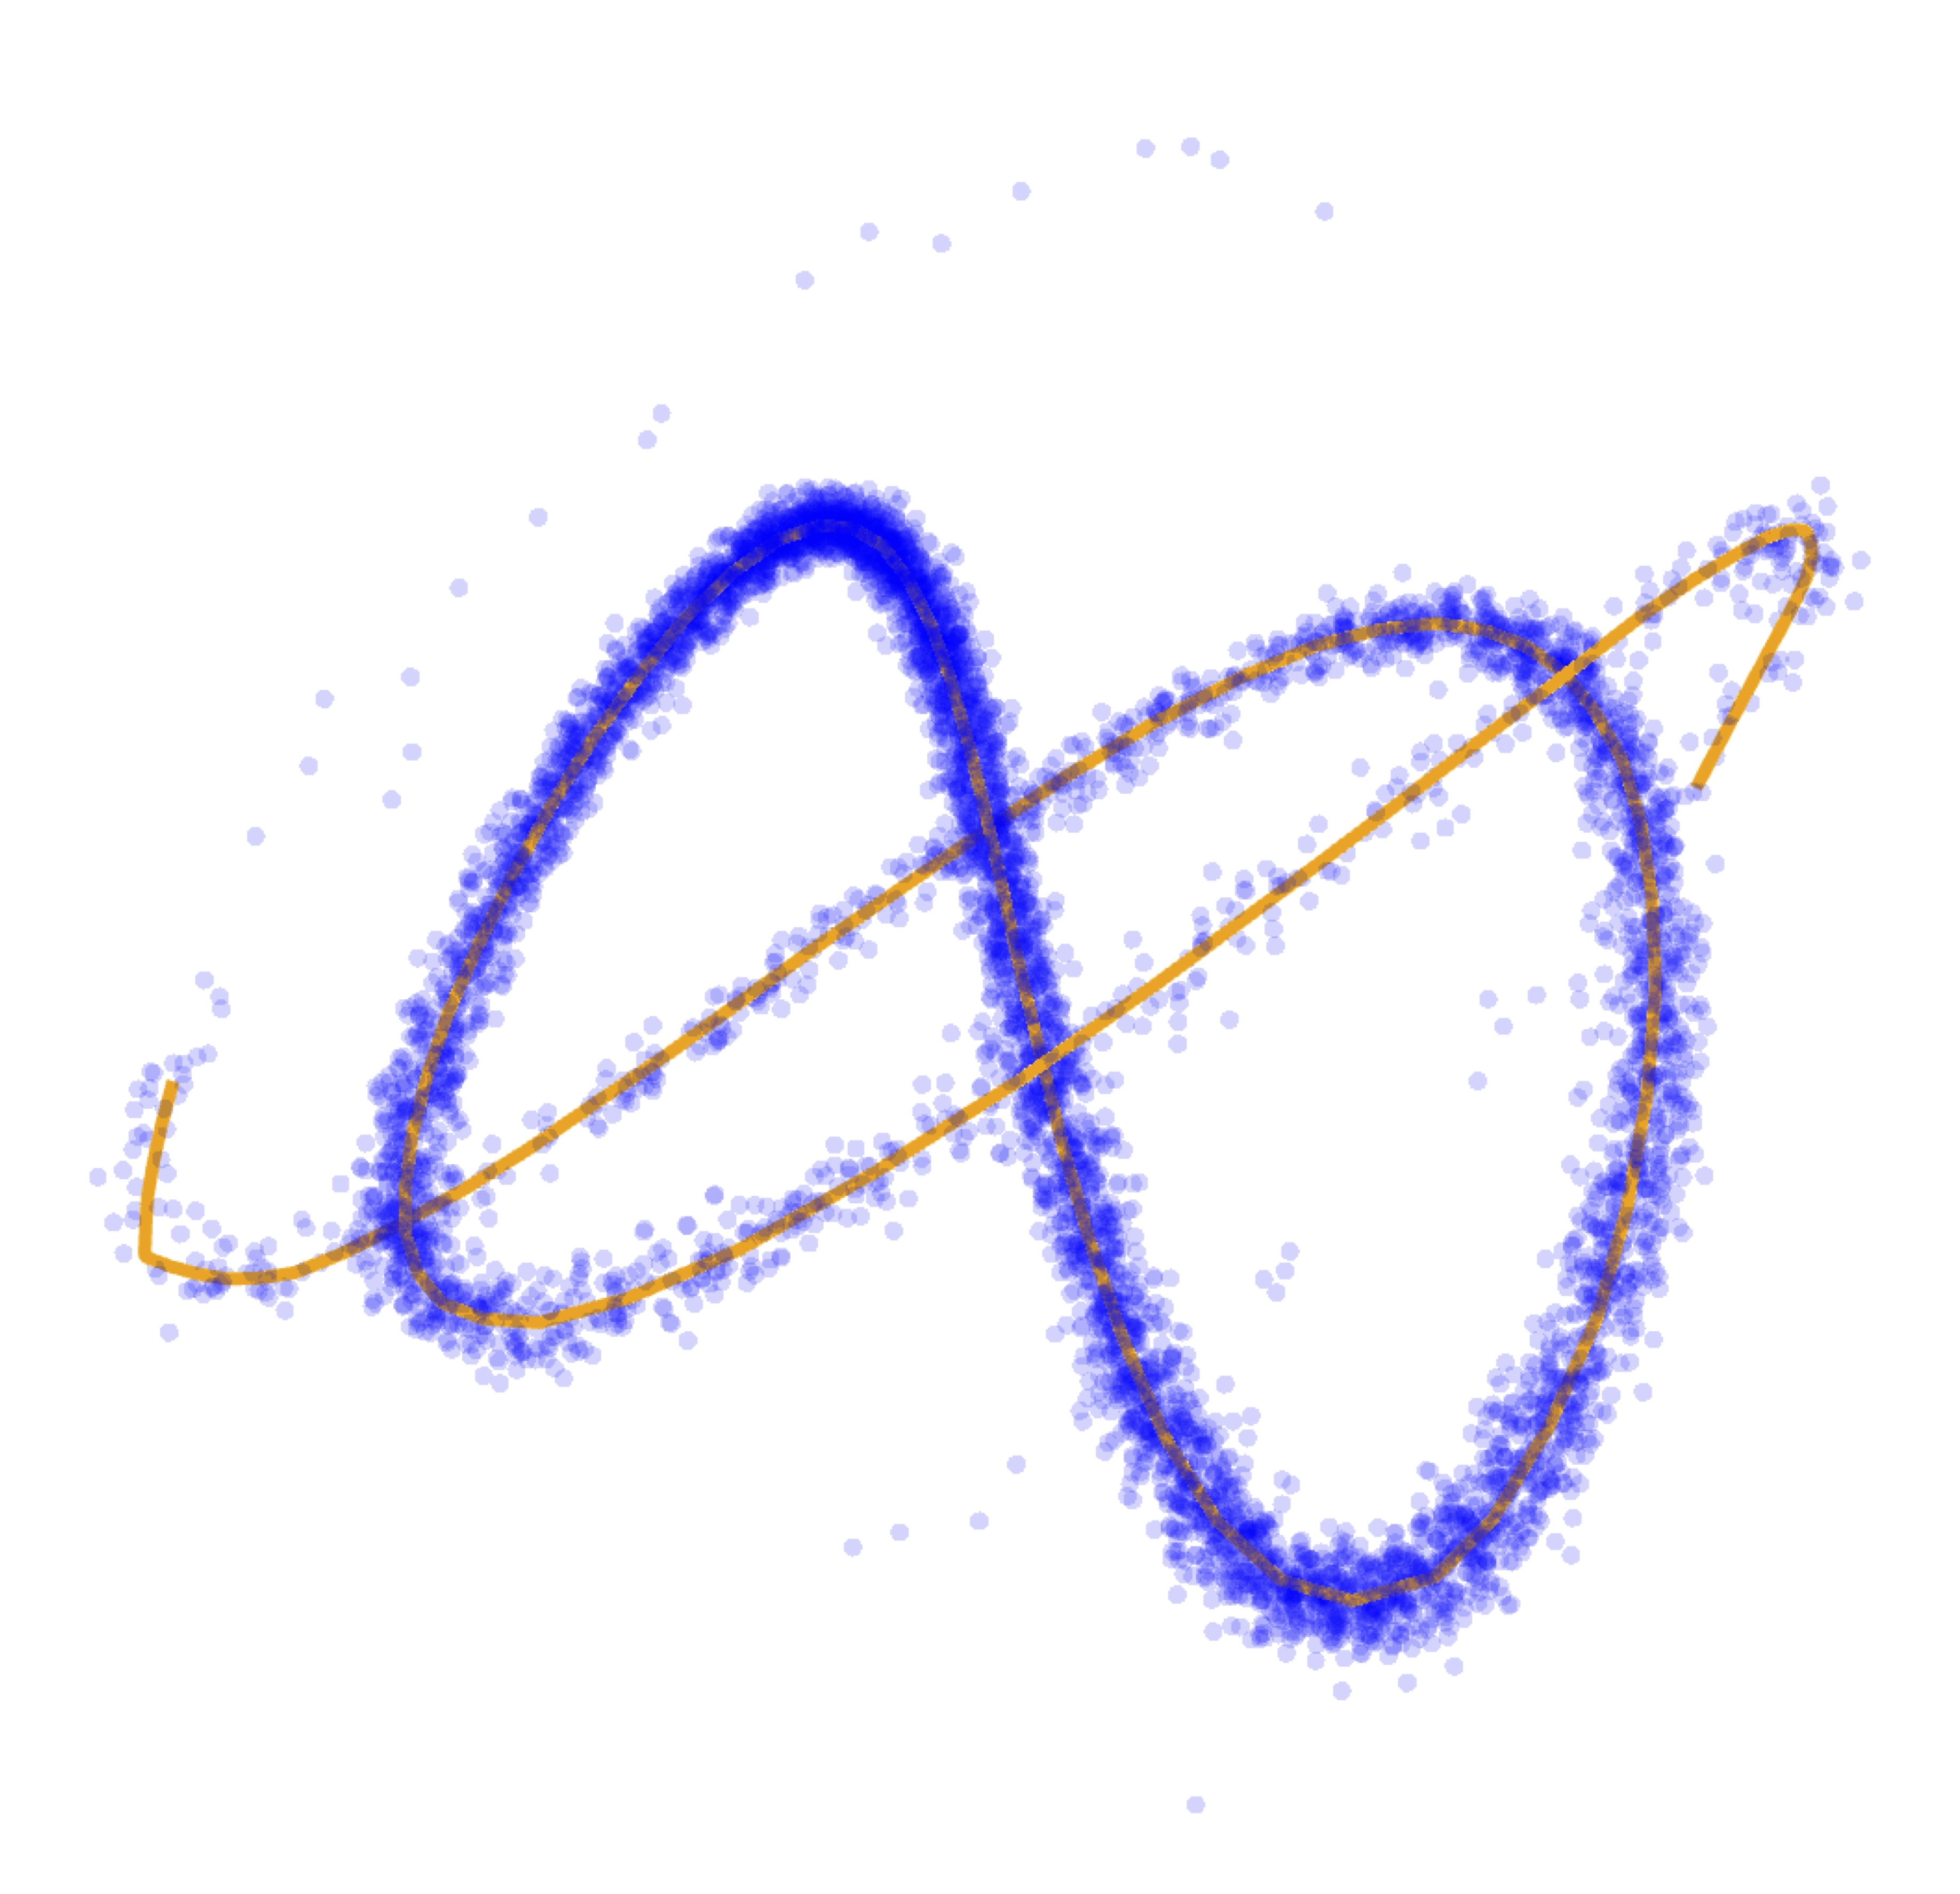
\includegraphics[width=\textwidth]{Chapter5/results/visualisations/RAE/projections/sinusoid_1_100/more_transparent/5_59_92.jpg}
        \caption{Dims (5, 59, 92)}
    \end{subfigure}
    \hfill
    \begin{subfigure}[t]{0.30\textwidth}
        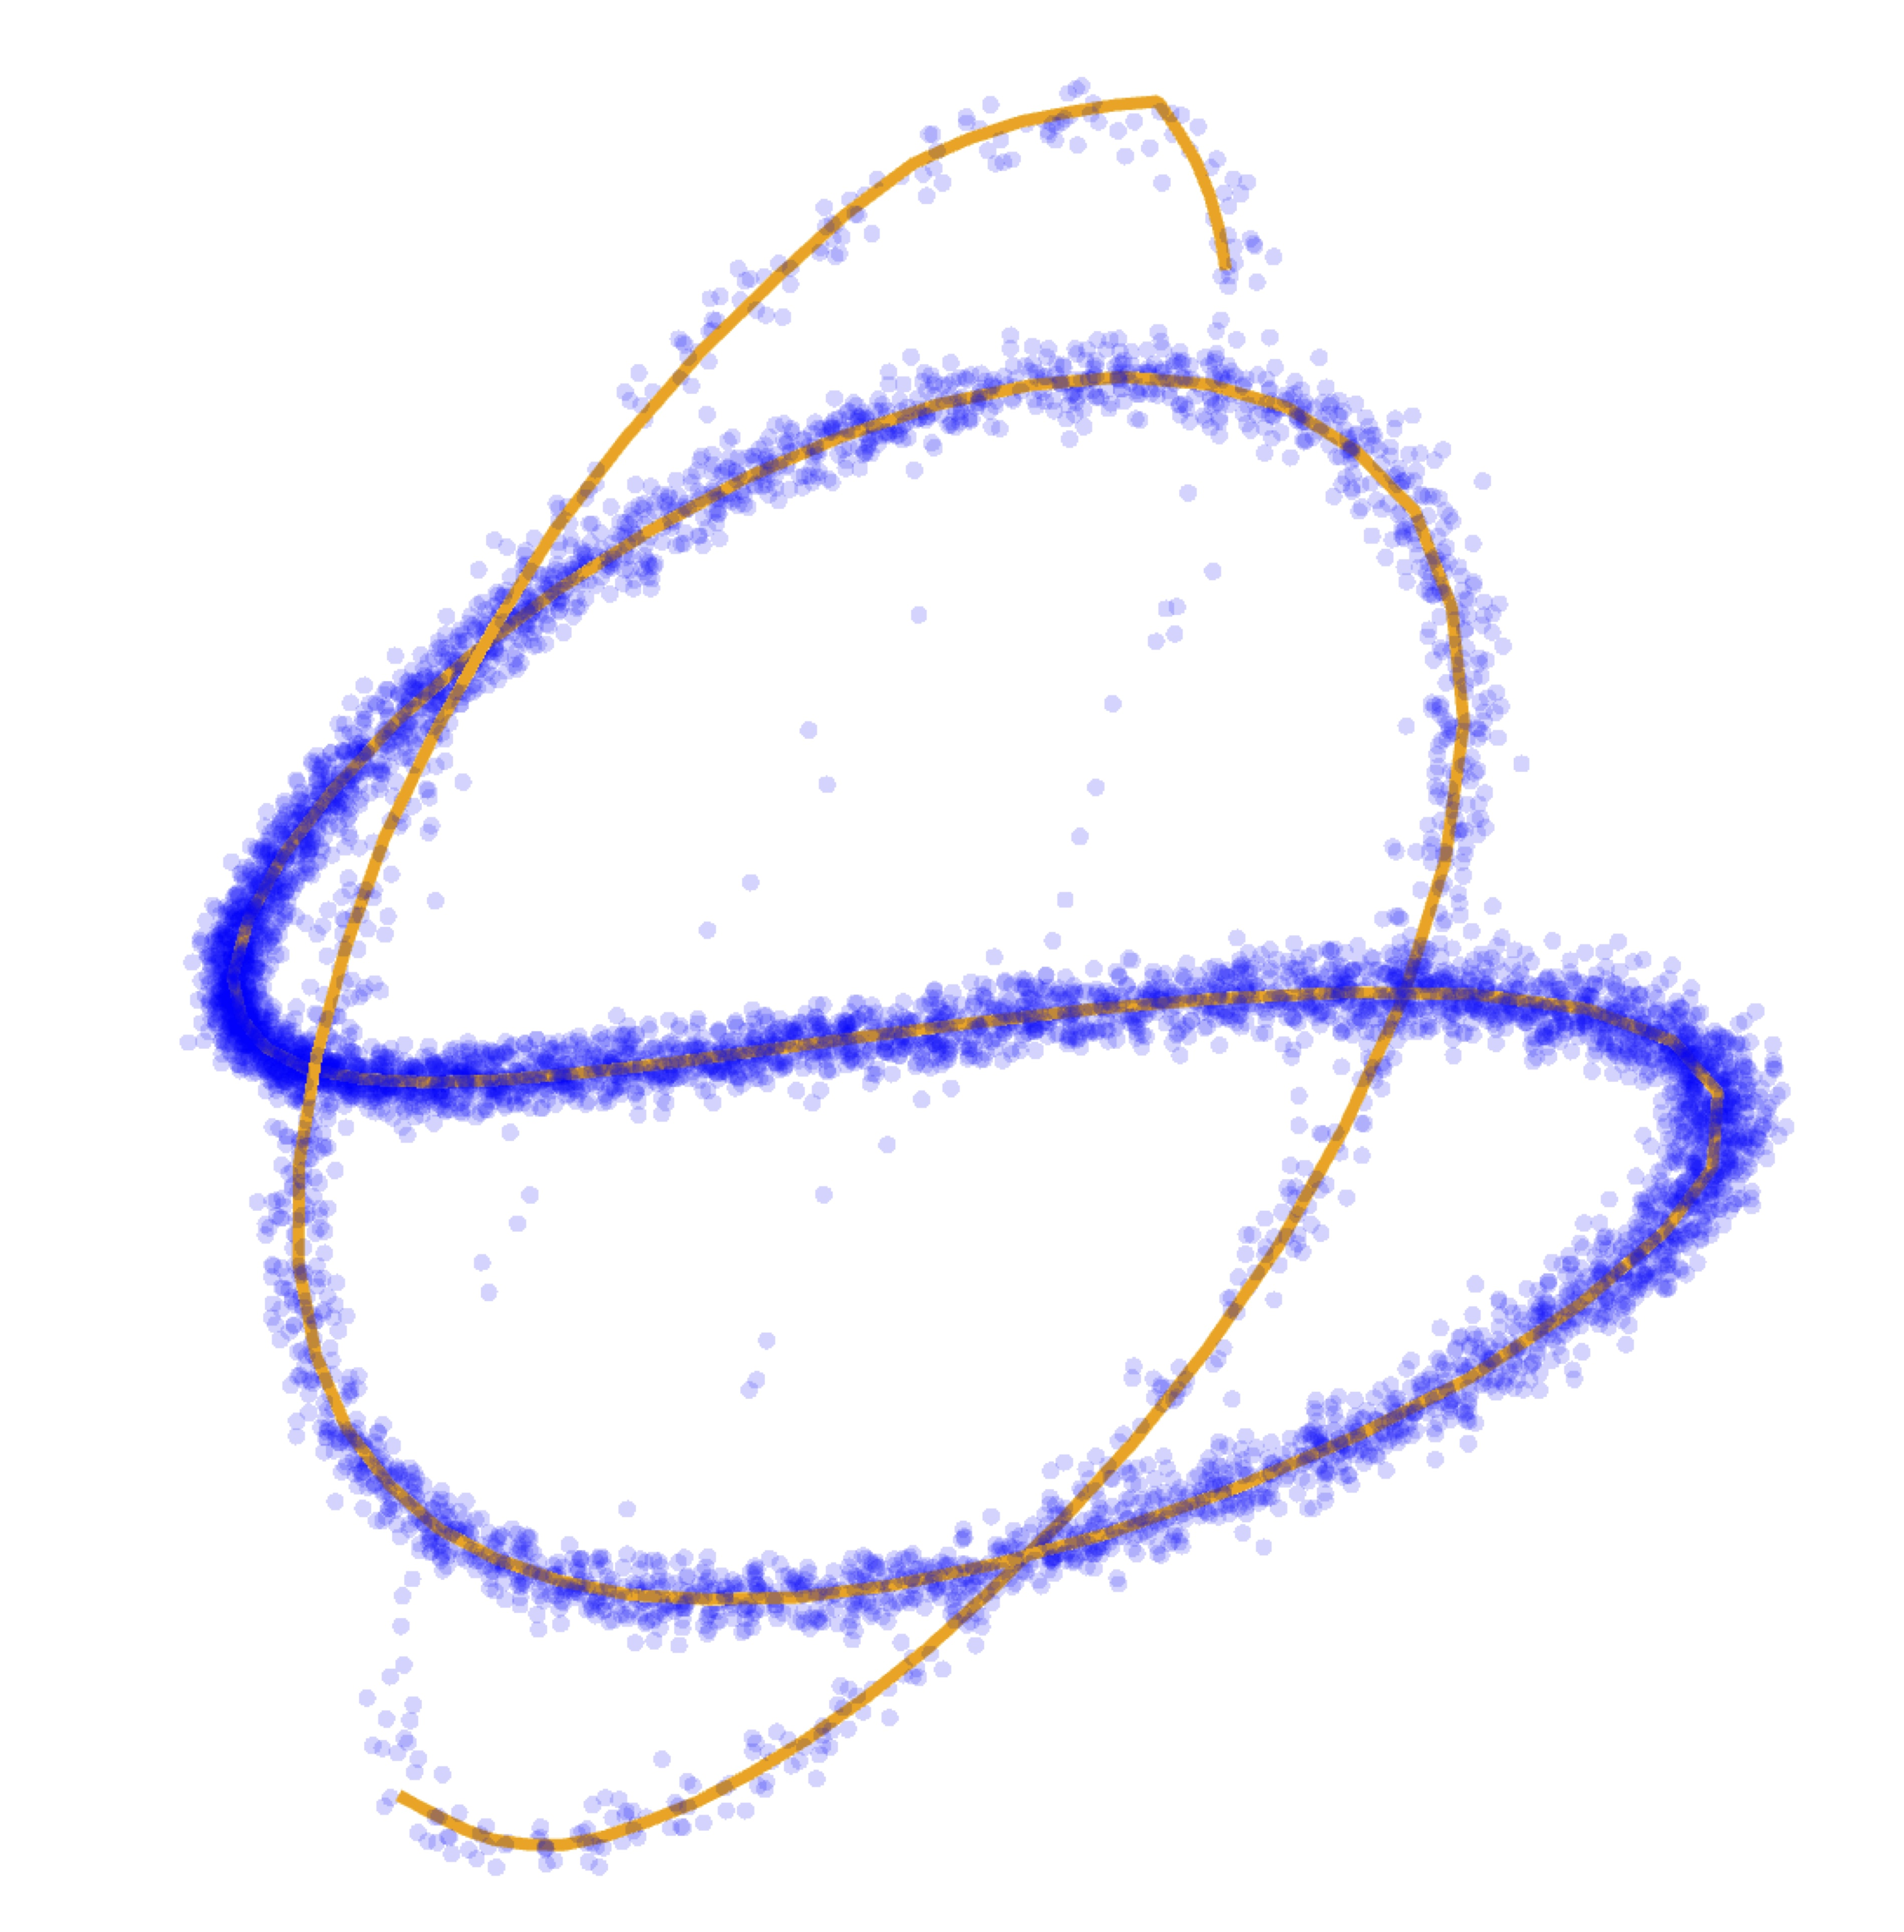
\includegraphics[width=\textwidth]{Chapter5/results/visualisations/RAE/projections/sinusoid_1_100/more_transparent/31_55_66.jpg}
        \caption{Dims (31, 55, 66)}
    \end{subfigure}
    \hfill
    \begin{subfigure}[t]{0.30\textwidth}
        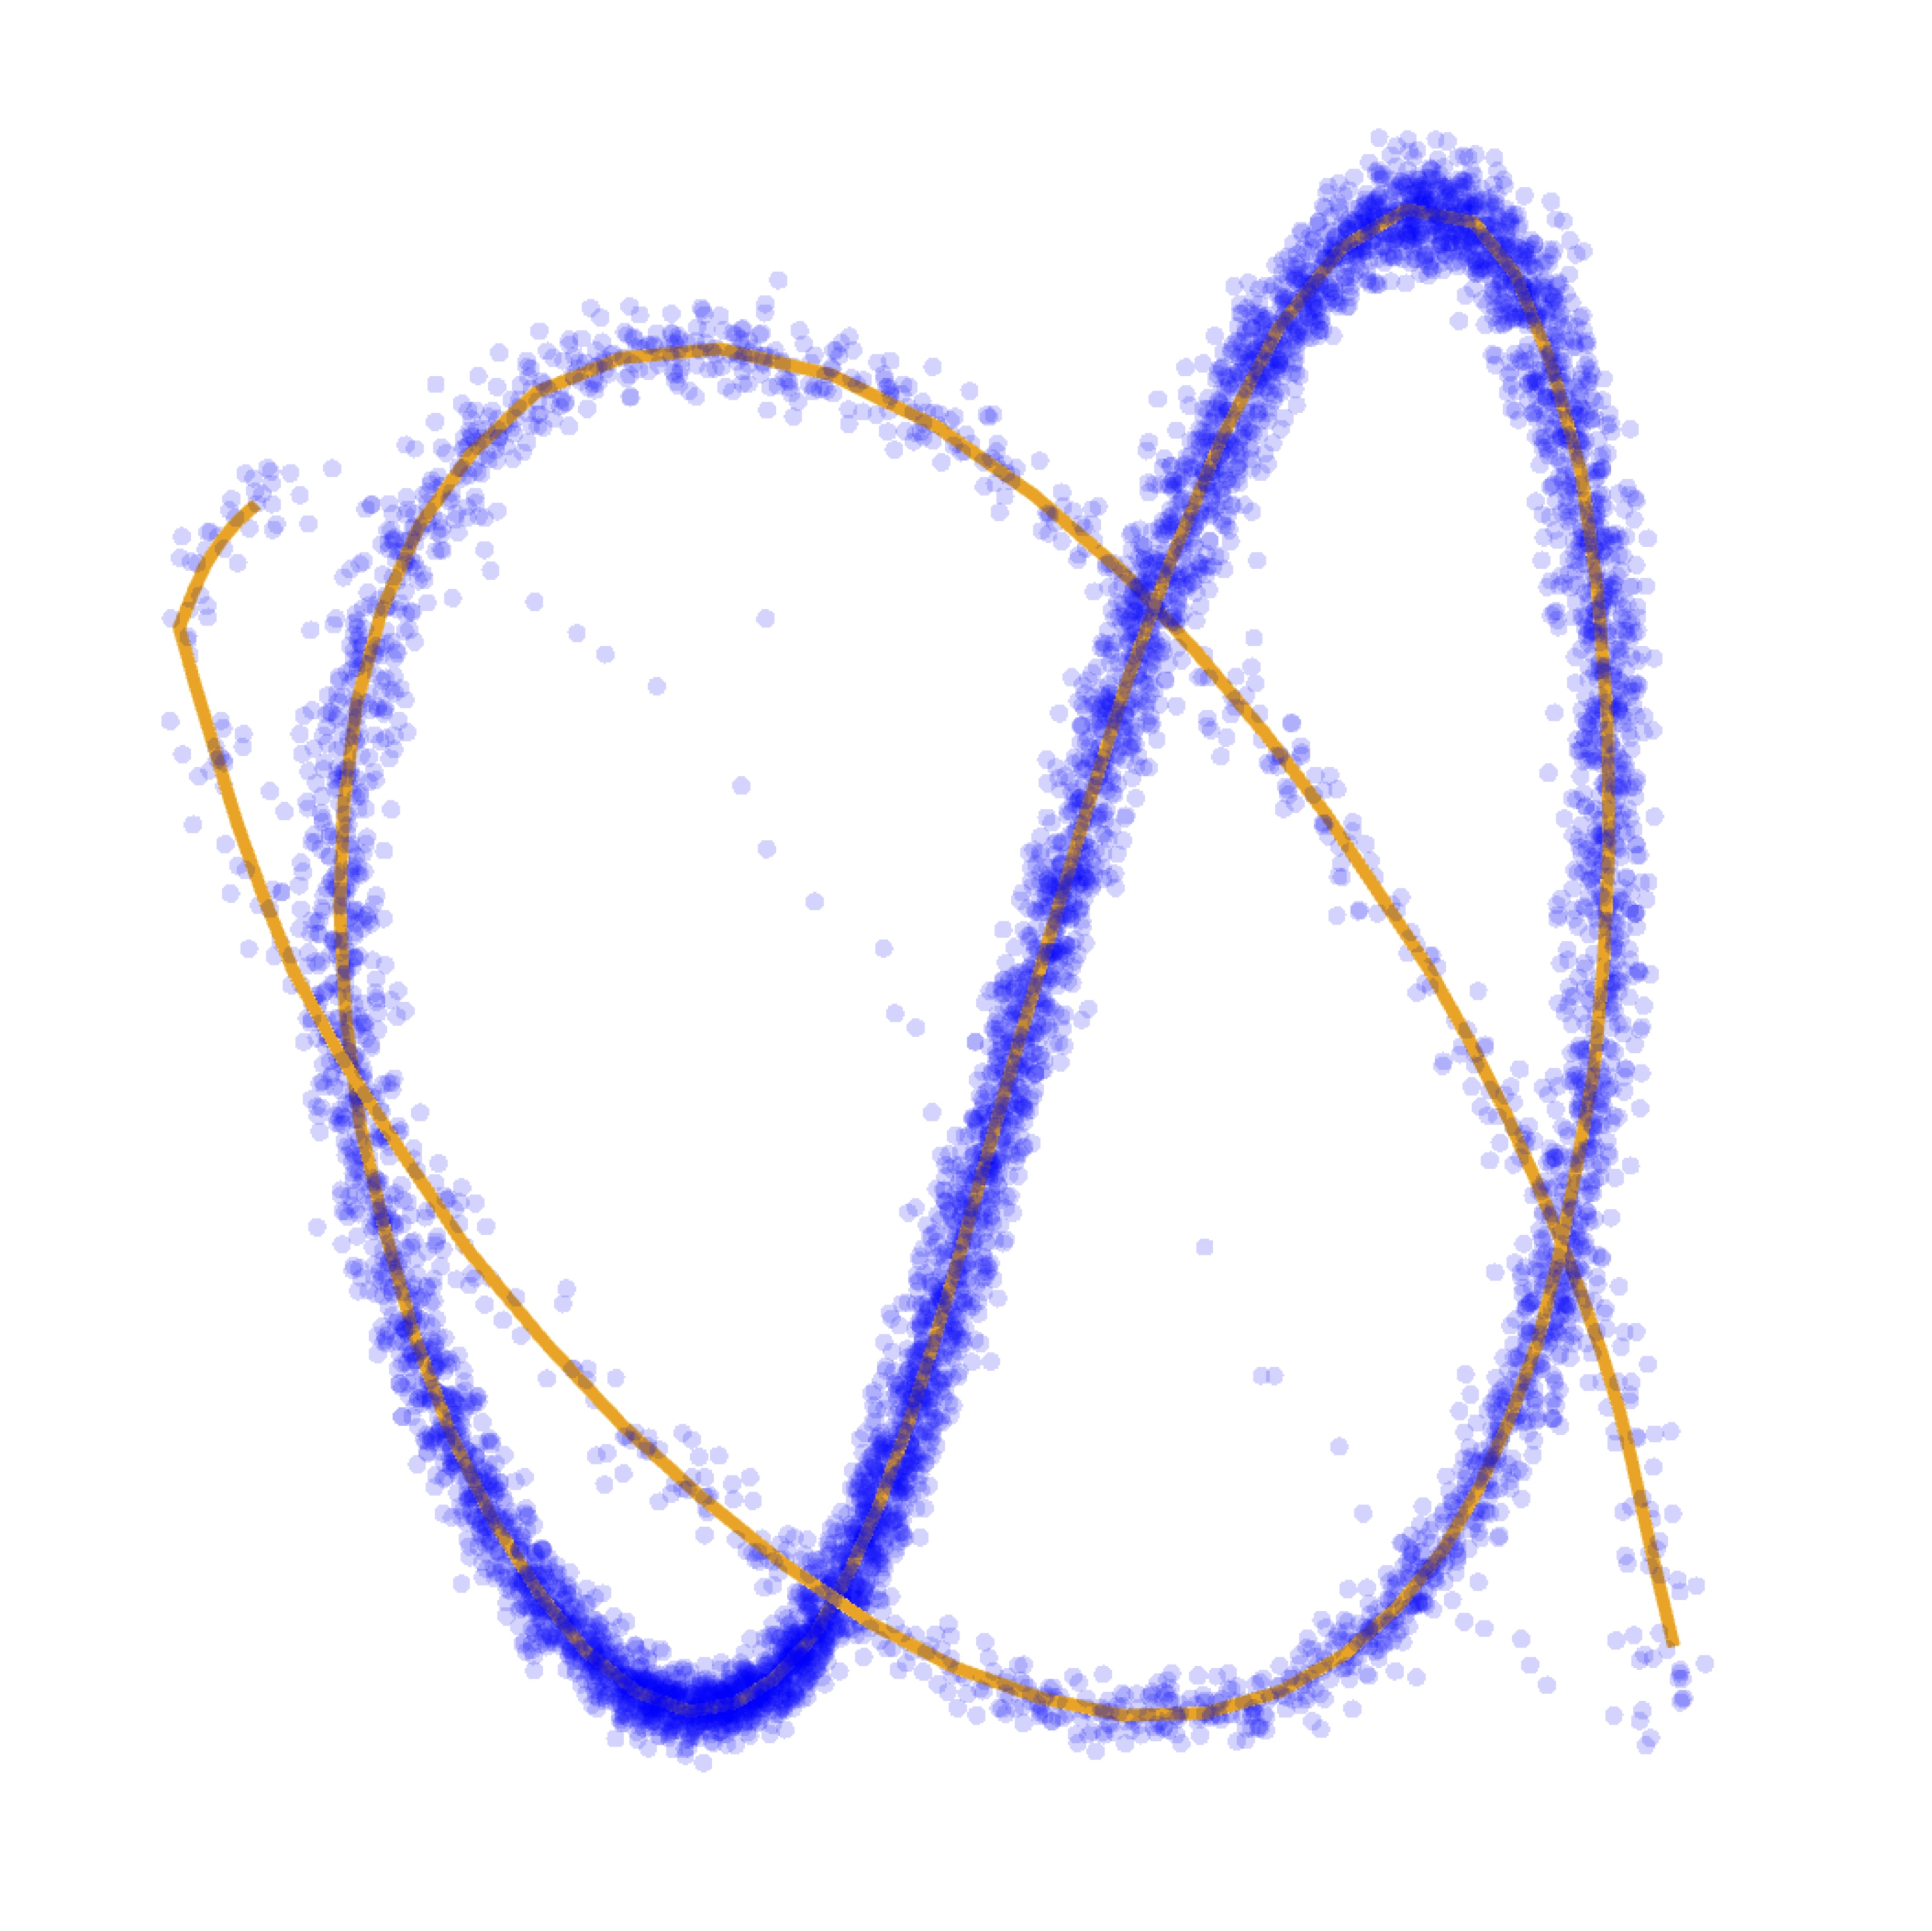
\includegraphics[width=\textwidth]{Chapter5/results/visualisations/RAE/projections/sinusoid_1_100/more_transparent/64_72_90.jpg}
        \caption{Dims (64, 72, 90)}
    \end{subfigure}

    % --- Middle Row: Hemisphere(5,20) ---
    \vspace{2em}
    \textbf{Hemisphere (5,20)} \par\vspace{0.4em}
    \begin{subfigure}[t]{0.43\textwidth}
        \centering
        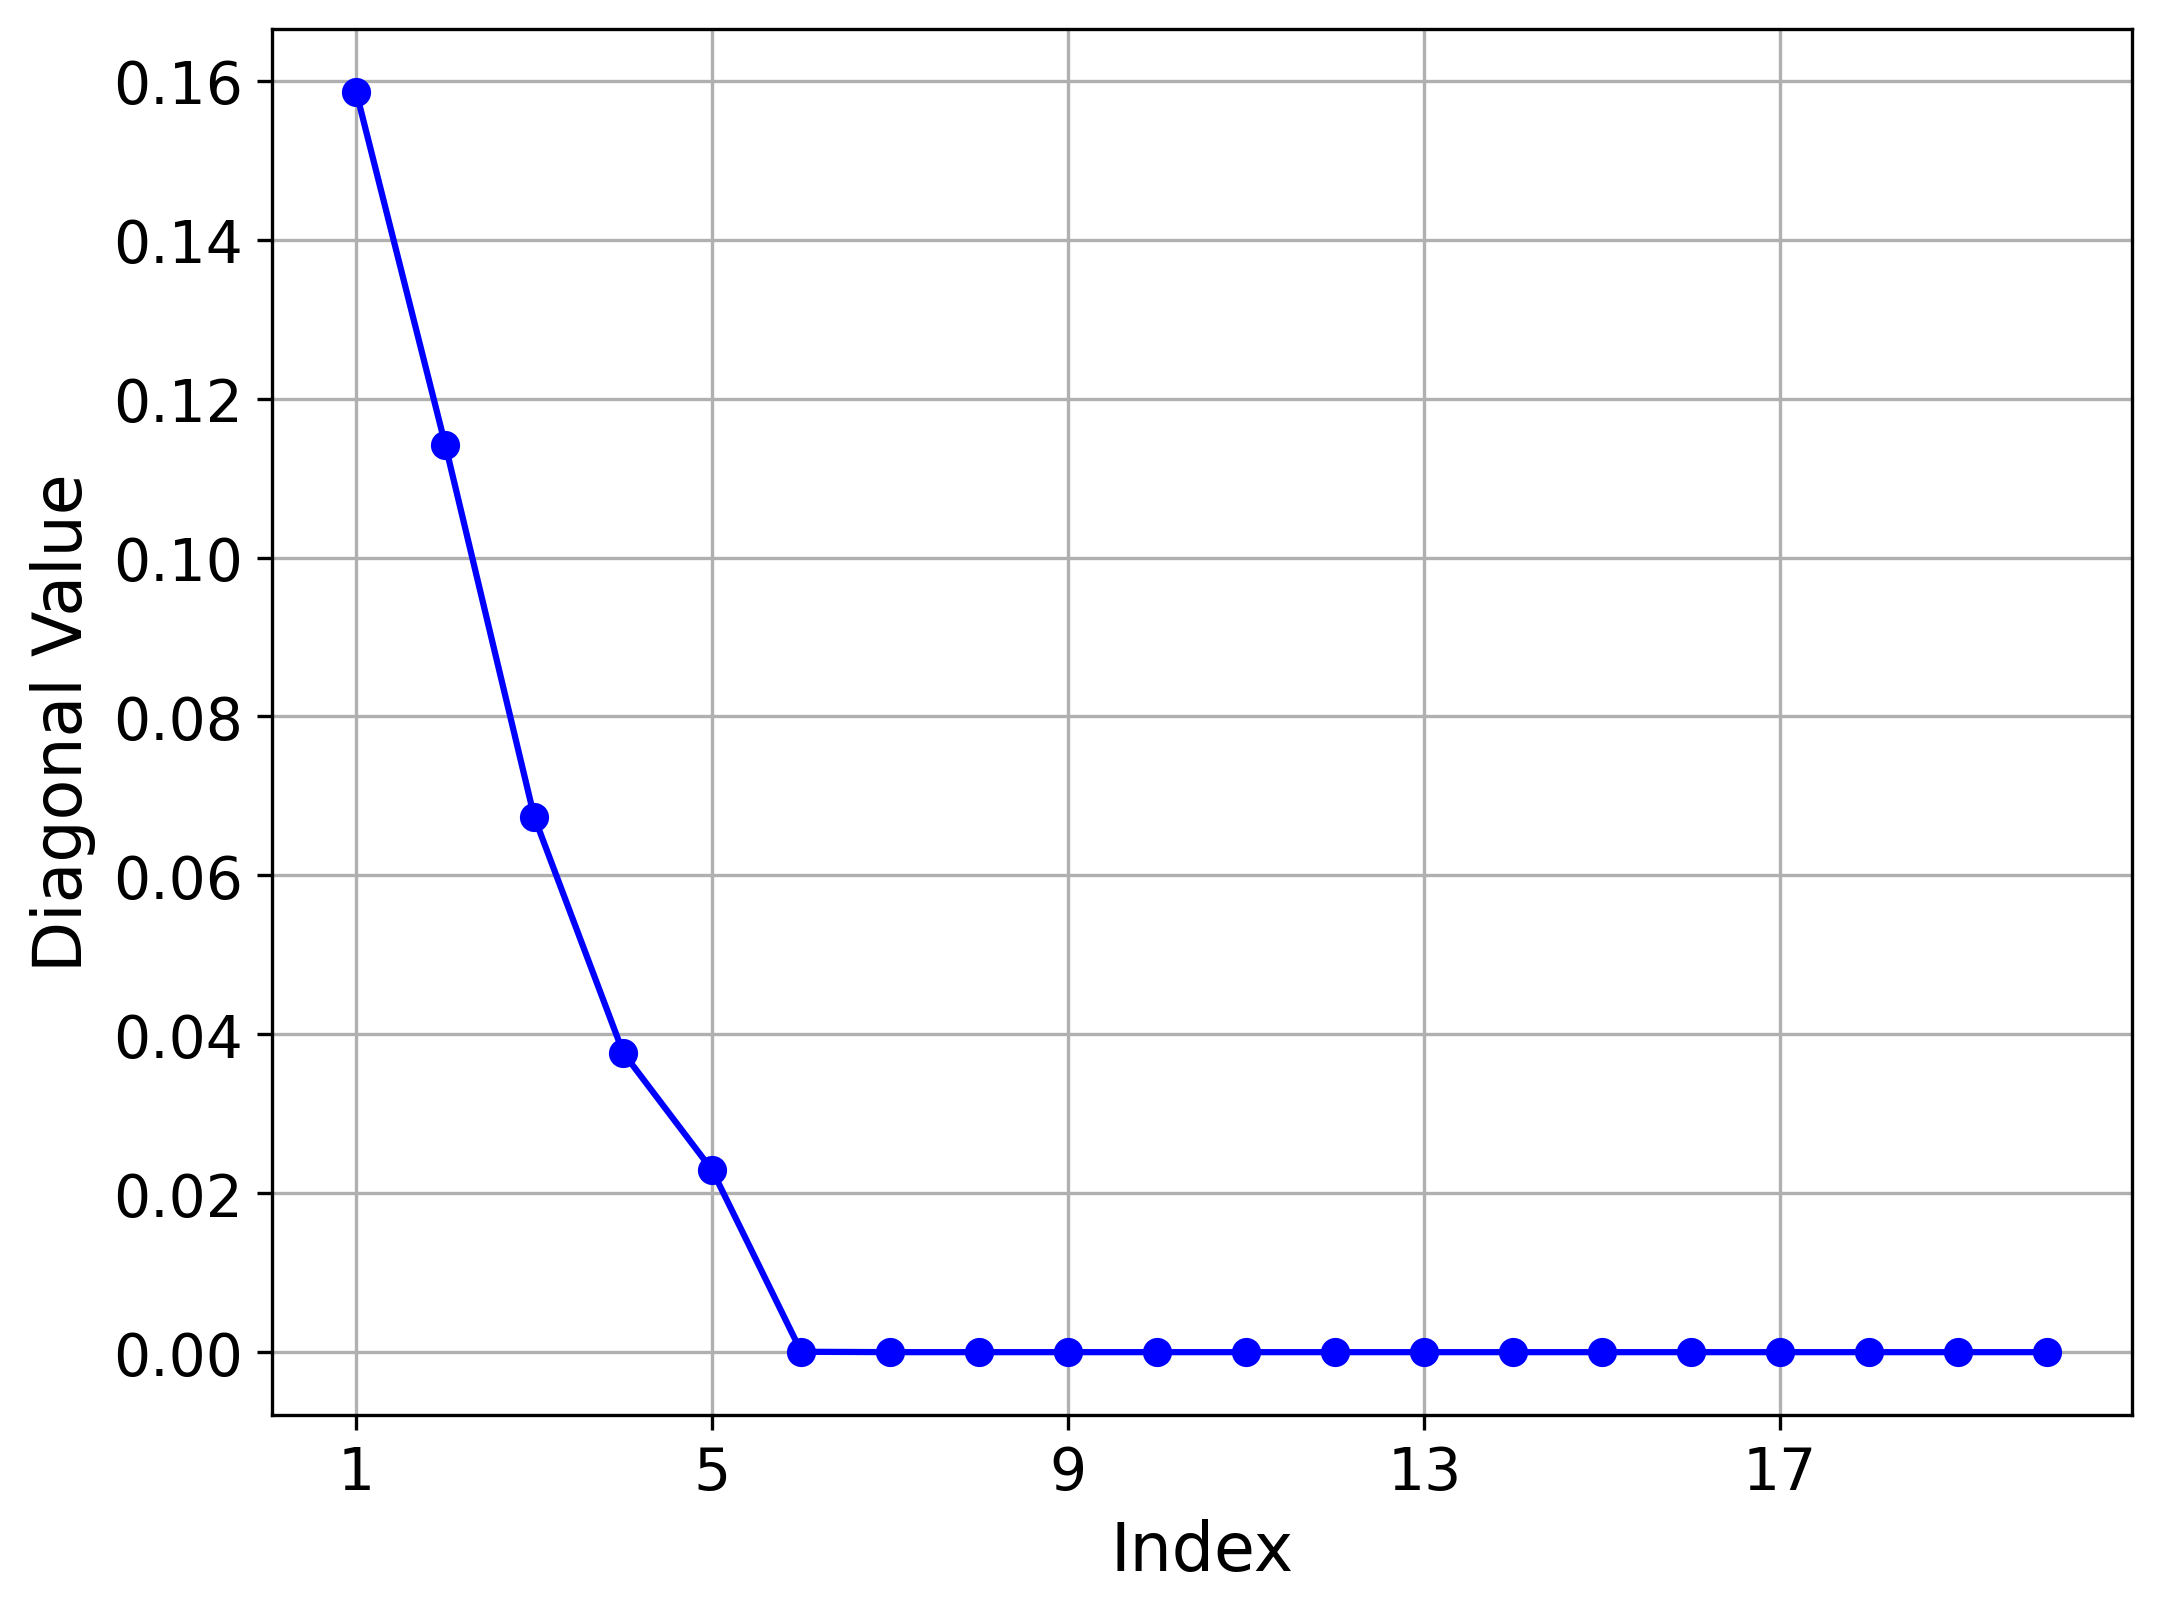
\includegraphics[width=\linewidth]{Chapter5/results/visualisations/RAE/reconstruction/hemisphere_5_20/diagonal_values_normal_scale.png}
        \caption{Learned variances (decreasing order).}
        \label{fig:hemisphere_variances}
    \end{subfigure}
    \hfill
    \begin{subfigure}[t]{0.53\textwidth}
        \centering
        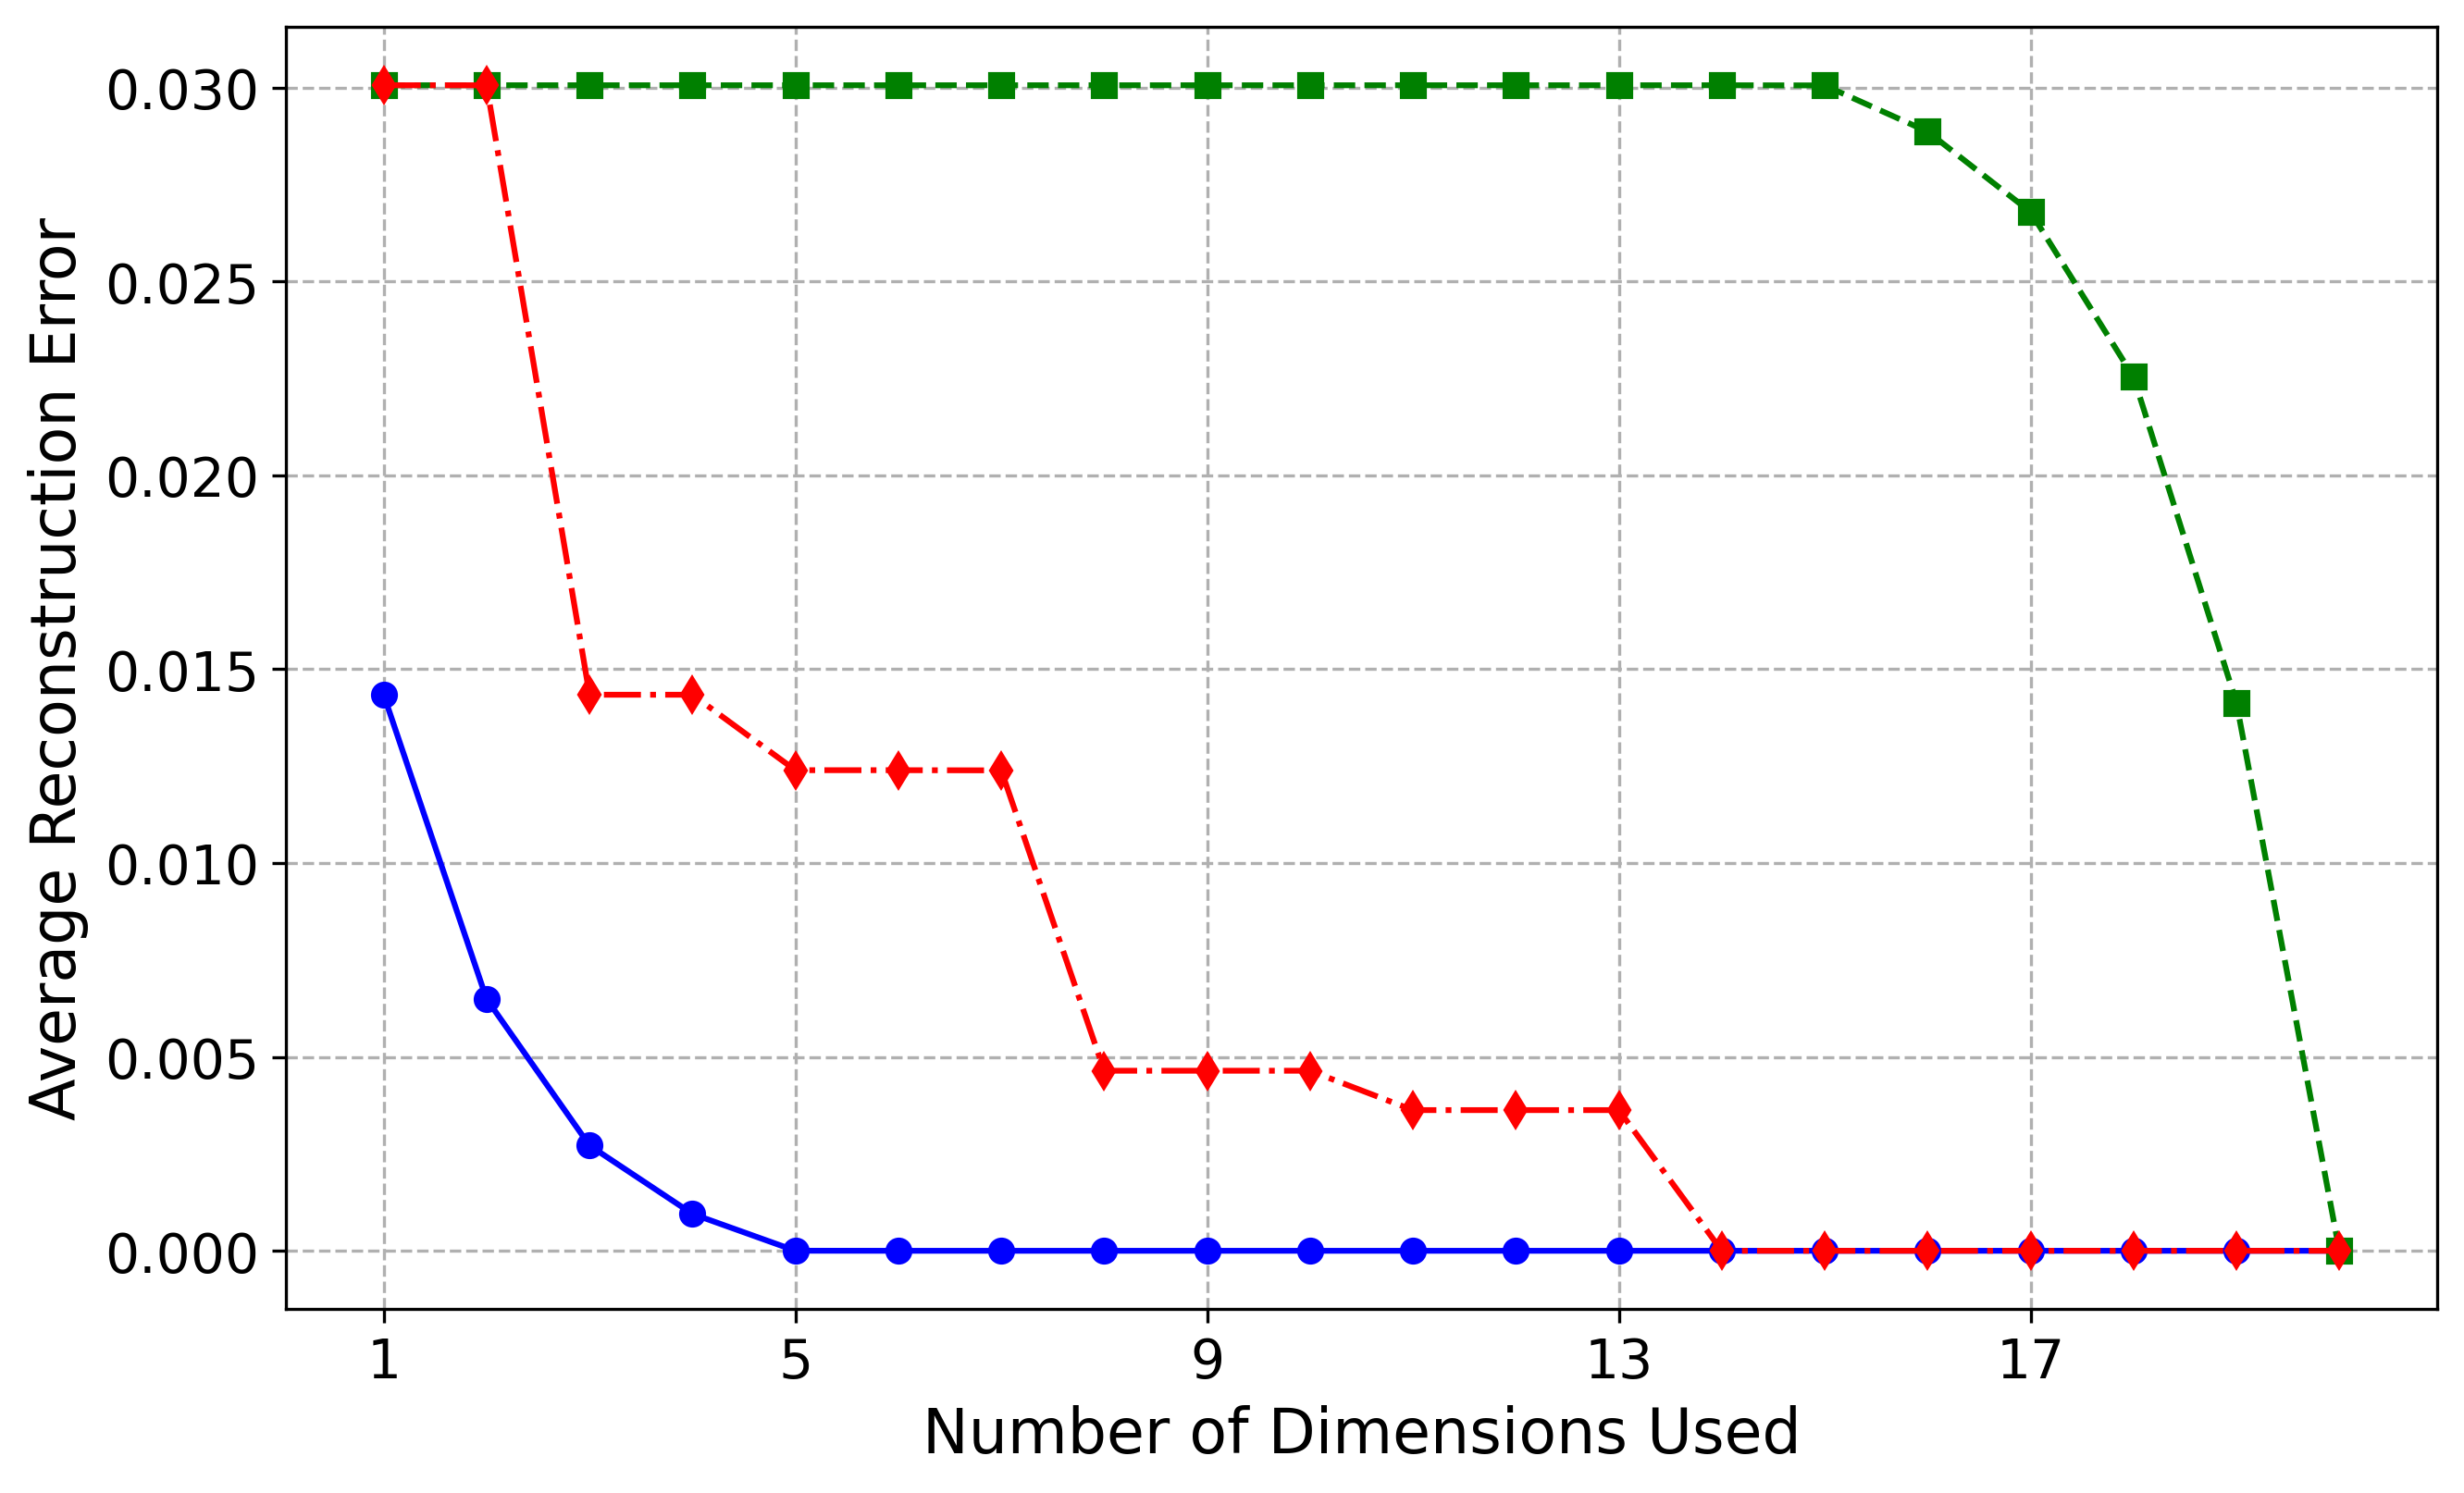
\includegraphics[width=\linewidth]{Chapter5/results/visualisations/RAE/reconstruction/hemisphere_5_20/reconstruction_error_plot_normal_scale.png}
        \caption{Reconstruction error for three latent orders.}
        \label{fig:hemisphere_reconstruction_errors}
    \end{subfigure}

    \vspace{1em}

    % --- Bottom Row: Sinusoid(5,20) ---
    \textbf{Sinusoid (5,20)} \par\vspace{0.4em}
    \begin{subfigure}[t]{0.43\textwidth}
        \centering
        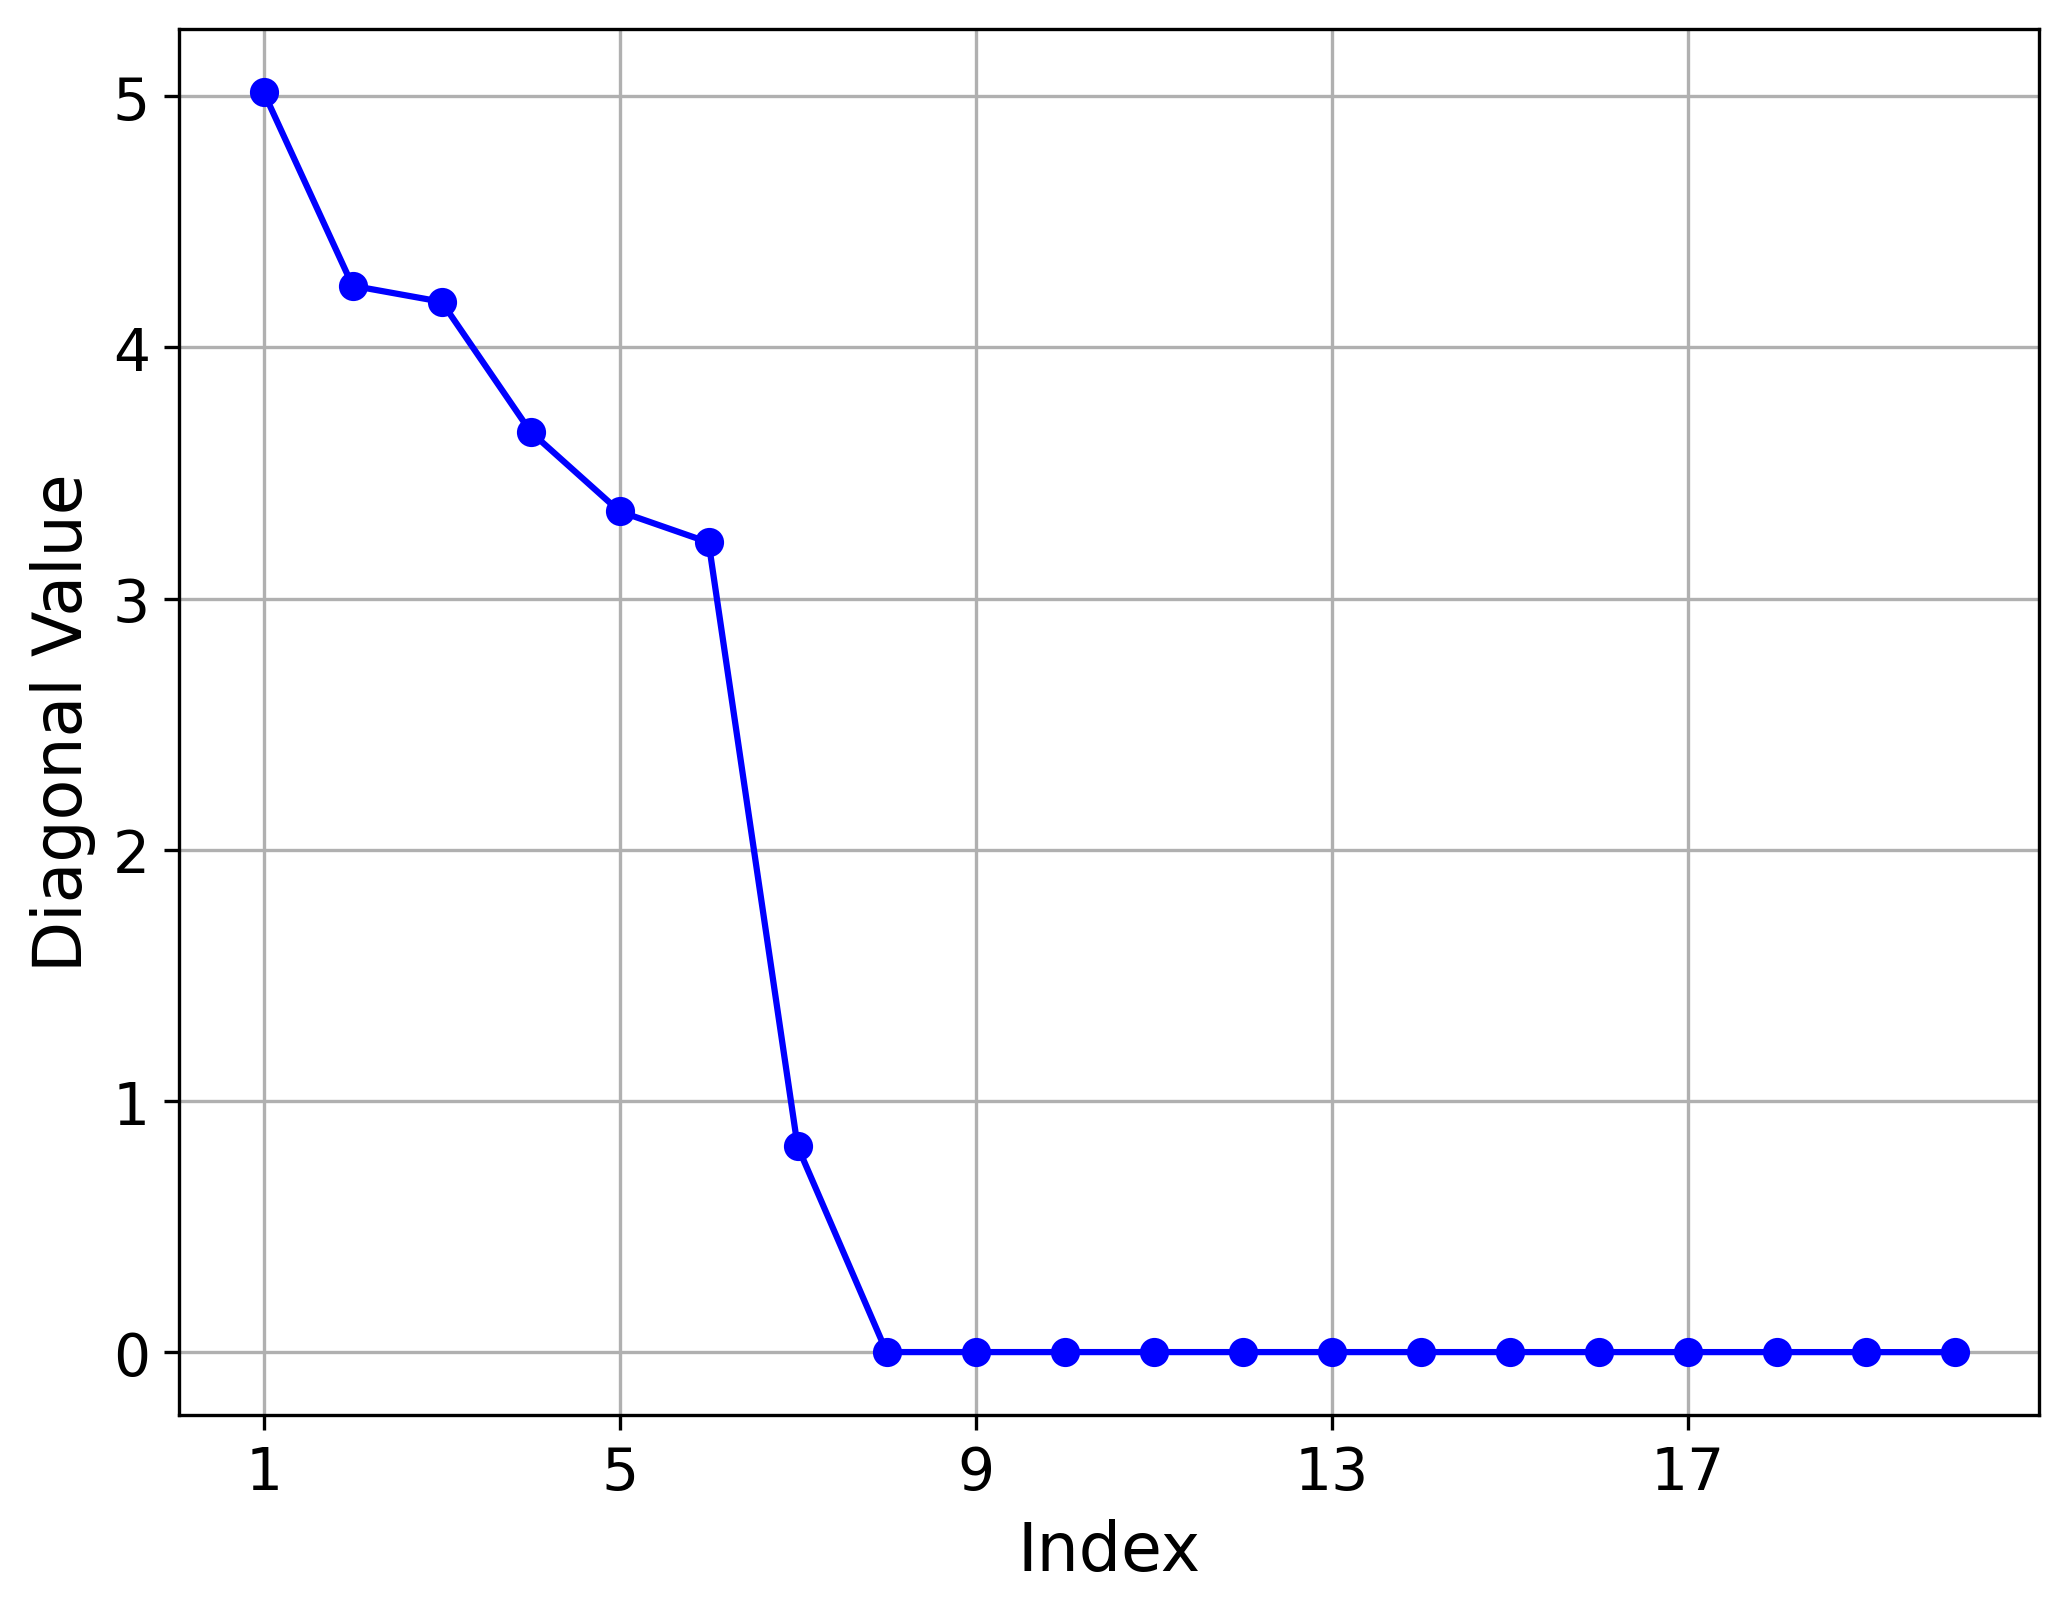
\includegraphics[width=\linewidth]{Chapter5/results/visualisations/RAE/reconstruction/sinusoid_5_20/diagonal_values_normal_scale.png}
        \caption{Learned variances (decreasing order).}
        \label{fig:sinusoid_variances}
    \end{subfigure}
    \hfill
    \begin{subfigure}[t]{0.53\textwidth}
        \centering
        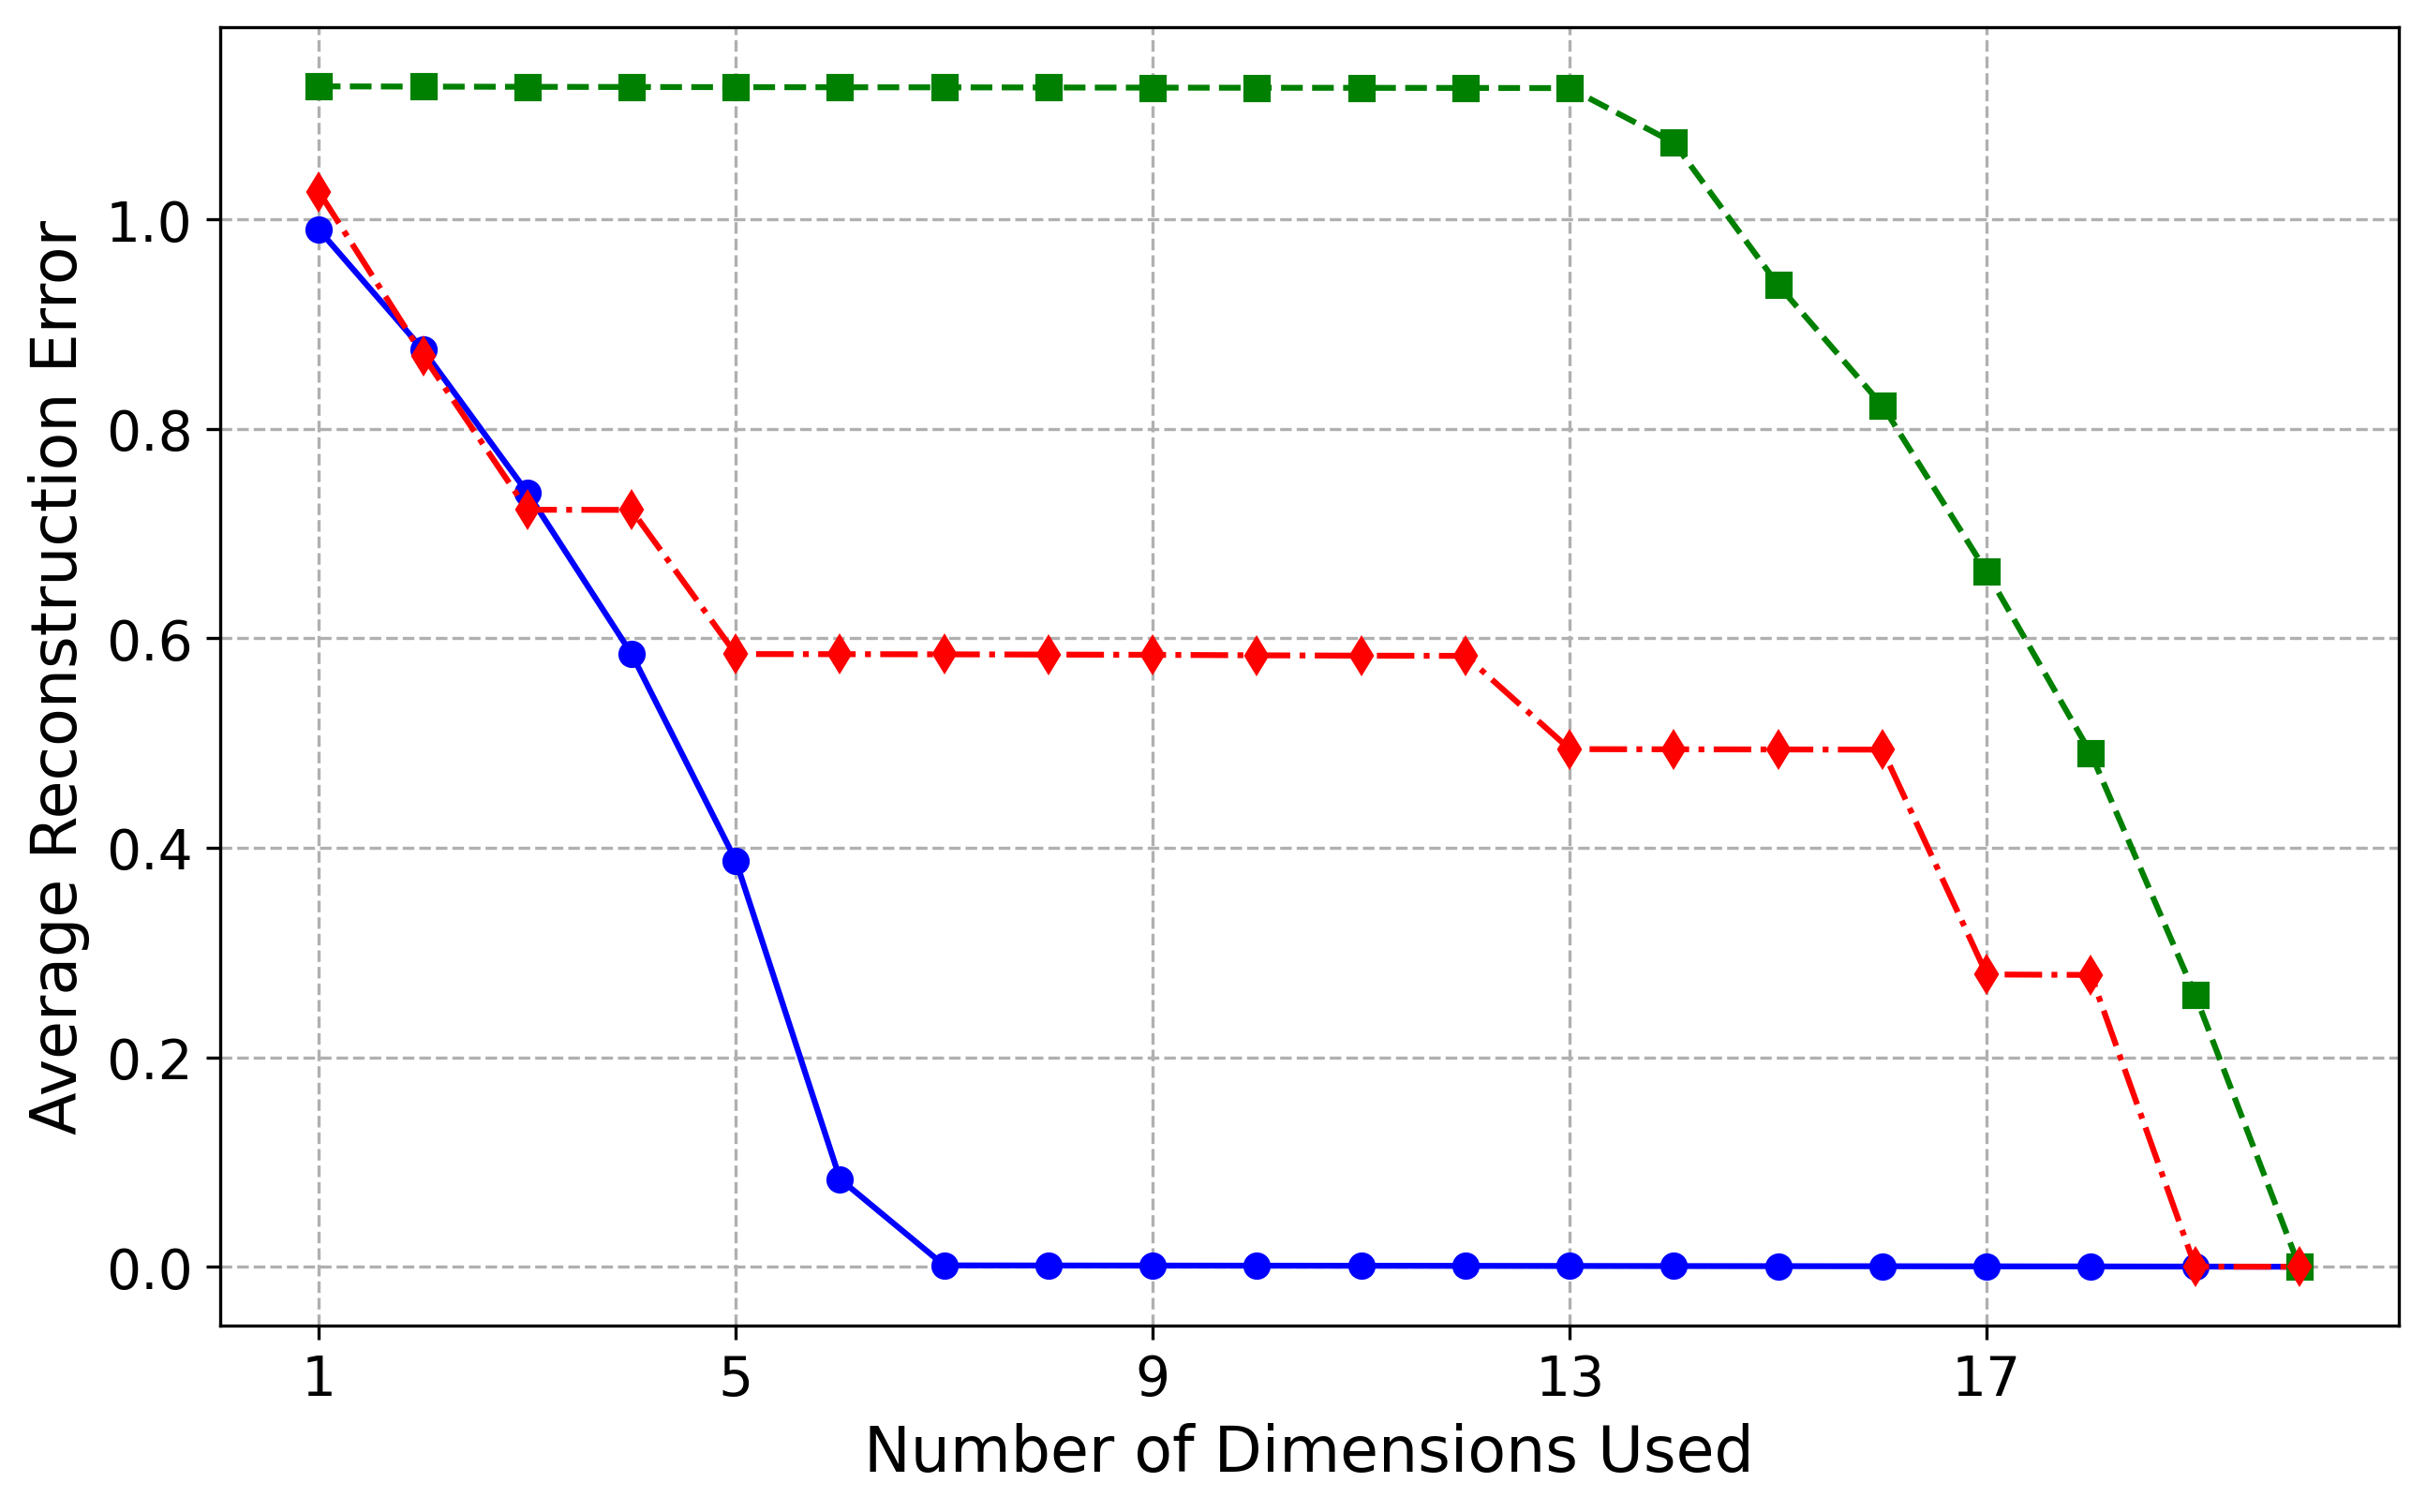
\includegraphics[width=\linewidth]{Chapter5/results/visualisations/RAE/reconstruction/sinusoid_5_20/reconstruction_error_plot_normal_scale.png}
        \caption{Reconstruction error for three latent orders.}
        \label{fig:sinusoid_reconstruction_errors}
    \end{subfigure}

    \caption{
    \textbf{Top:} Approximate data manifold learned by the Riemannian autoencoder for Sinusoid(1, 100).Orange curves depict the learned manifold; blue points indicate training data.
    \textbf{Bottom:} Learned variances and reconstruction errors for Hemisphere(5,20) and Sinusoid(5,20). Left: learned variances in decreasing order. Right: average $\ell^2$ reconstruction error versus the number of latent dimensions used. Errors are shown for three variance-based orderings: \textbf{blue} (decreasing), \textbf{green} (increasing), and \textbf{red} (random).}
    \label{fig:rae_appendix_combined}
\end{figure}

\clearpage
\section{Error Metrics for Evaluation of Pullback Geometries}
\label{app:Error metrics for evaluation of Pullback Geometries}

\paragraph{Geodesic Error.}
The geodesic error measures the difference between geodesics on the learned and ground truth pullback manifolds. Given two points \(\mathbf{x}_0, \mathbf{x}_1 \in \mathbb{R}^{\dimInd}\), let \(\gamma_{\mathbf{x}_0, \mathbf{x}_1}^{\diffeo_{\theta_2}}(t)\) and \(\gamma_{\mathbf{x}_0, \mathbf{x}_1}^{\diffeo_{\mathrm{GT}}}(t)\) denote the geodesics induced by the learned map \(\diffeo_{\theta_2}\) and the ground truth map \(\diffeo_{\mathrm{GT}}\), respectively, where \(t \in [0, 1]\).

The geodesic error is calculated as the mean Euclidean distance between the learned and ground truth geodesics over \(N\) pairs of points:

\[
\text{Geodesic Error} = \frac{1}{N} \sum_{i=1}^{N} \frac{1}{T} \sum_{k=1}^{T} \left\| \gamma_{\mathbf{x}_0^{(i)}, \mathbf{x}_1^{(i)}}^{\diffeo_{\theta_2}}(t_k) - \gamma_{\mathbf{x}_0^{(i)}, \mathbf{x}_1^{(i)}}^{\diffeo_{\mathrm{GT}}}(t_k) \right\|_2,
\]
where \(T\) is the number of time steps used to discretize the geodesic, and \(t_k = \frac{k-1}{T-1}\) for \(k = 1, \dots, T\).

This metric captures the average discrepancy between the learned and ground truth geodesics, reflecting the accuracy of the learned pullback manifold.

\paragraph{Variation Error.}
The variation error quantifies the sensitivity of the geodesic computation under small perturbations to one of the endpoints. For two points \(\mathbf{x}_0, \mathbf{x}_1 \in \mathbb{R}^{\dimInd}\), let \(\mathbf{z} = \mathbf{x}_1 + \Delta\mathbf{x}\), where \(\Delta\mathbf{x}\) is a random variable sampled from the Gaussian distribution:

\[
\Delta\mathbf{x} \sim \mathcal{N}(\mathbf{0}, 0.1^2 \mathbf{I}),
\]

with mean \(\mathbf{0}\) and covariance \(0.1^2 \mathbf{I}\), where \(\mathbf{I}\) is the identity matrix. Define \(\gamma_{\mathbf{x}_0, \mathbf{x}_1}^{\diffeo_{\theta_2}}(t)\) and \(\gamma_{\mathbf{x}_0, \mathbf{z}}^{\diffeo_{\theta_2}}(t)\) as the geodesics from \(\mathbf{x}_0\) to \(\mathbf{x}_1\) and \(\mathbf{z}\), respectively, induced by the learned map \(\diffeo_{\theta_2}\).

The variation error is calculated as the mean Euclidean distance between the geodesic from \(\mathbf{x}_0\) to \(\mathbf{x}_1\) and the perturbed geodesic from \(\mathbf{x}_0\) to \(\mathbf{z}\):

\[
\text{Variation Error} = \frac{1}{N} \sum_{i=1}^{N} \frac{1}{T} \sum_{k=1}^{T} \left\| \gamma_{\mathbf{x}_0^{(i)}, \mathbf{x}_1^{(i)}}^{\diffeo_{\theta_2}}(t_k) - \gamma_{\mathbf{x}_0^{(i)}, \mathbf{z}^{(i)}}^{\diffeo_{\theta_2}}(t_k) \right\|_2,
\]

where \(N\) is the number of sampled point pairs, \(T\) is the number of time steps used to discretize the geodesic, and \(t_k = \frac{k-1}{T-1}\) for \(k = 1, \dots, T\).

This metric evaluates the robustness of the learned geodesic against small perturbations, providing insight into the stability of the learned manifold.


\section{Dataset Construction Details}
\label{app:dataset_construction}

In this section, we provide a detailed explanation of the construction of the datasets used in our experiments. We organize the datasets into two categories based on the experimental sections in which they are used.

\subsection{Datasets for Manifold Mapping Experiments}
\label{app:manifold_mapping}

\begin{figure}[ht]
\centering
\begin{subfigure}[b]{0.32\textwidth}
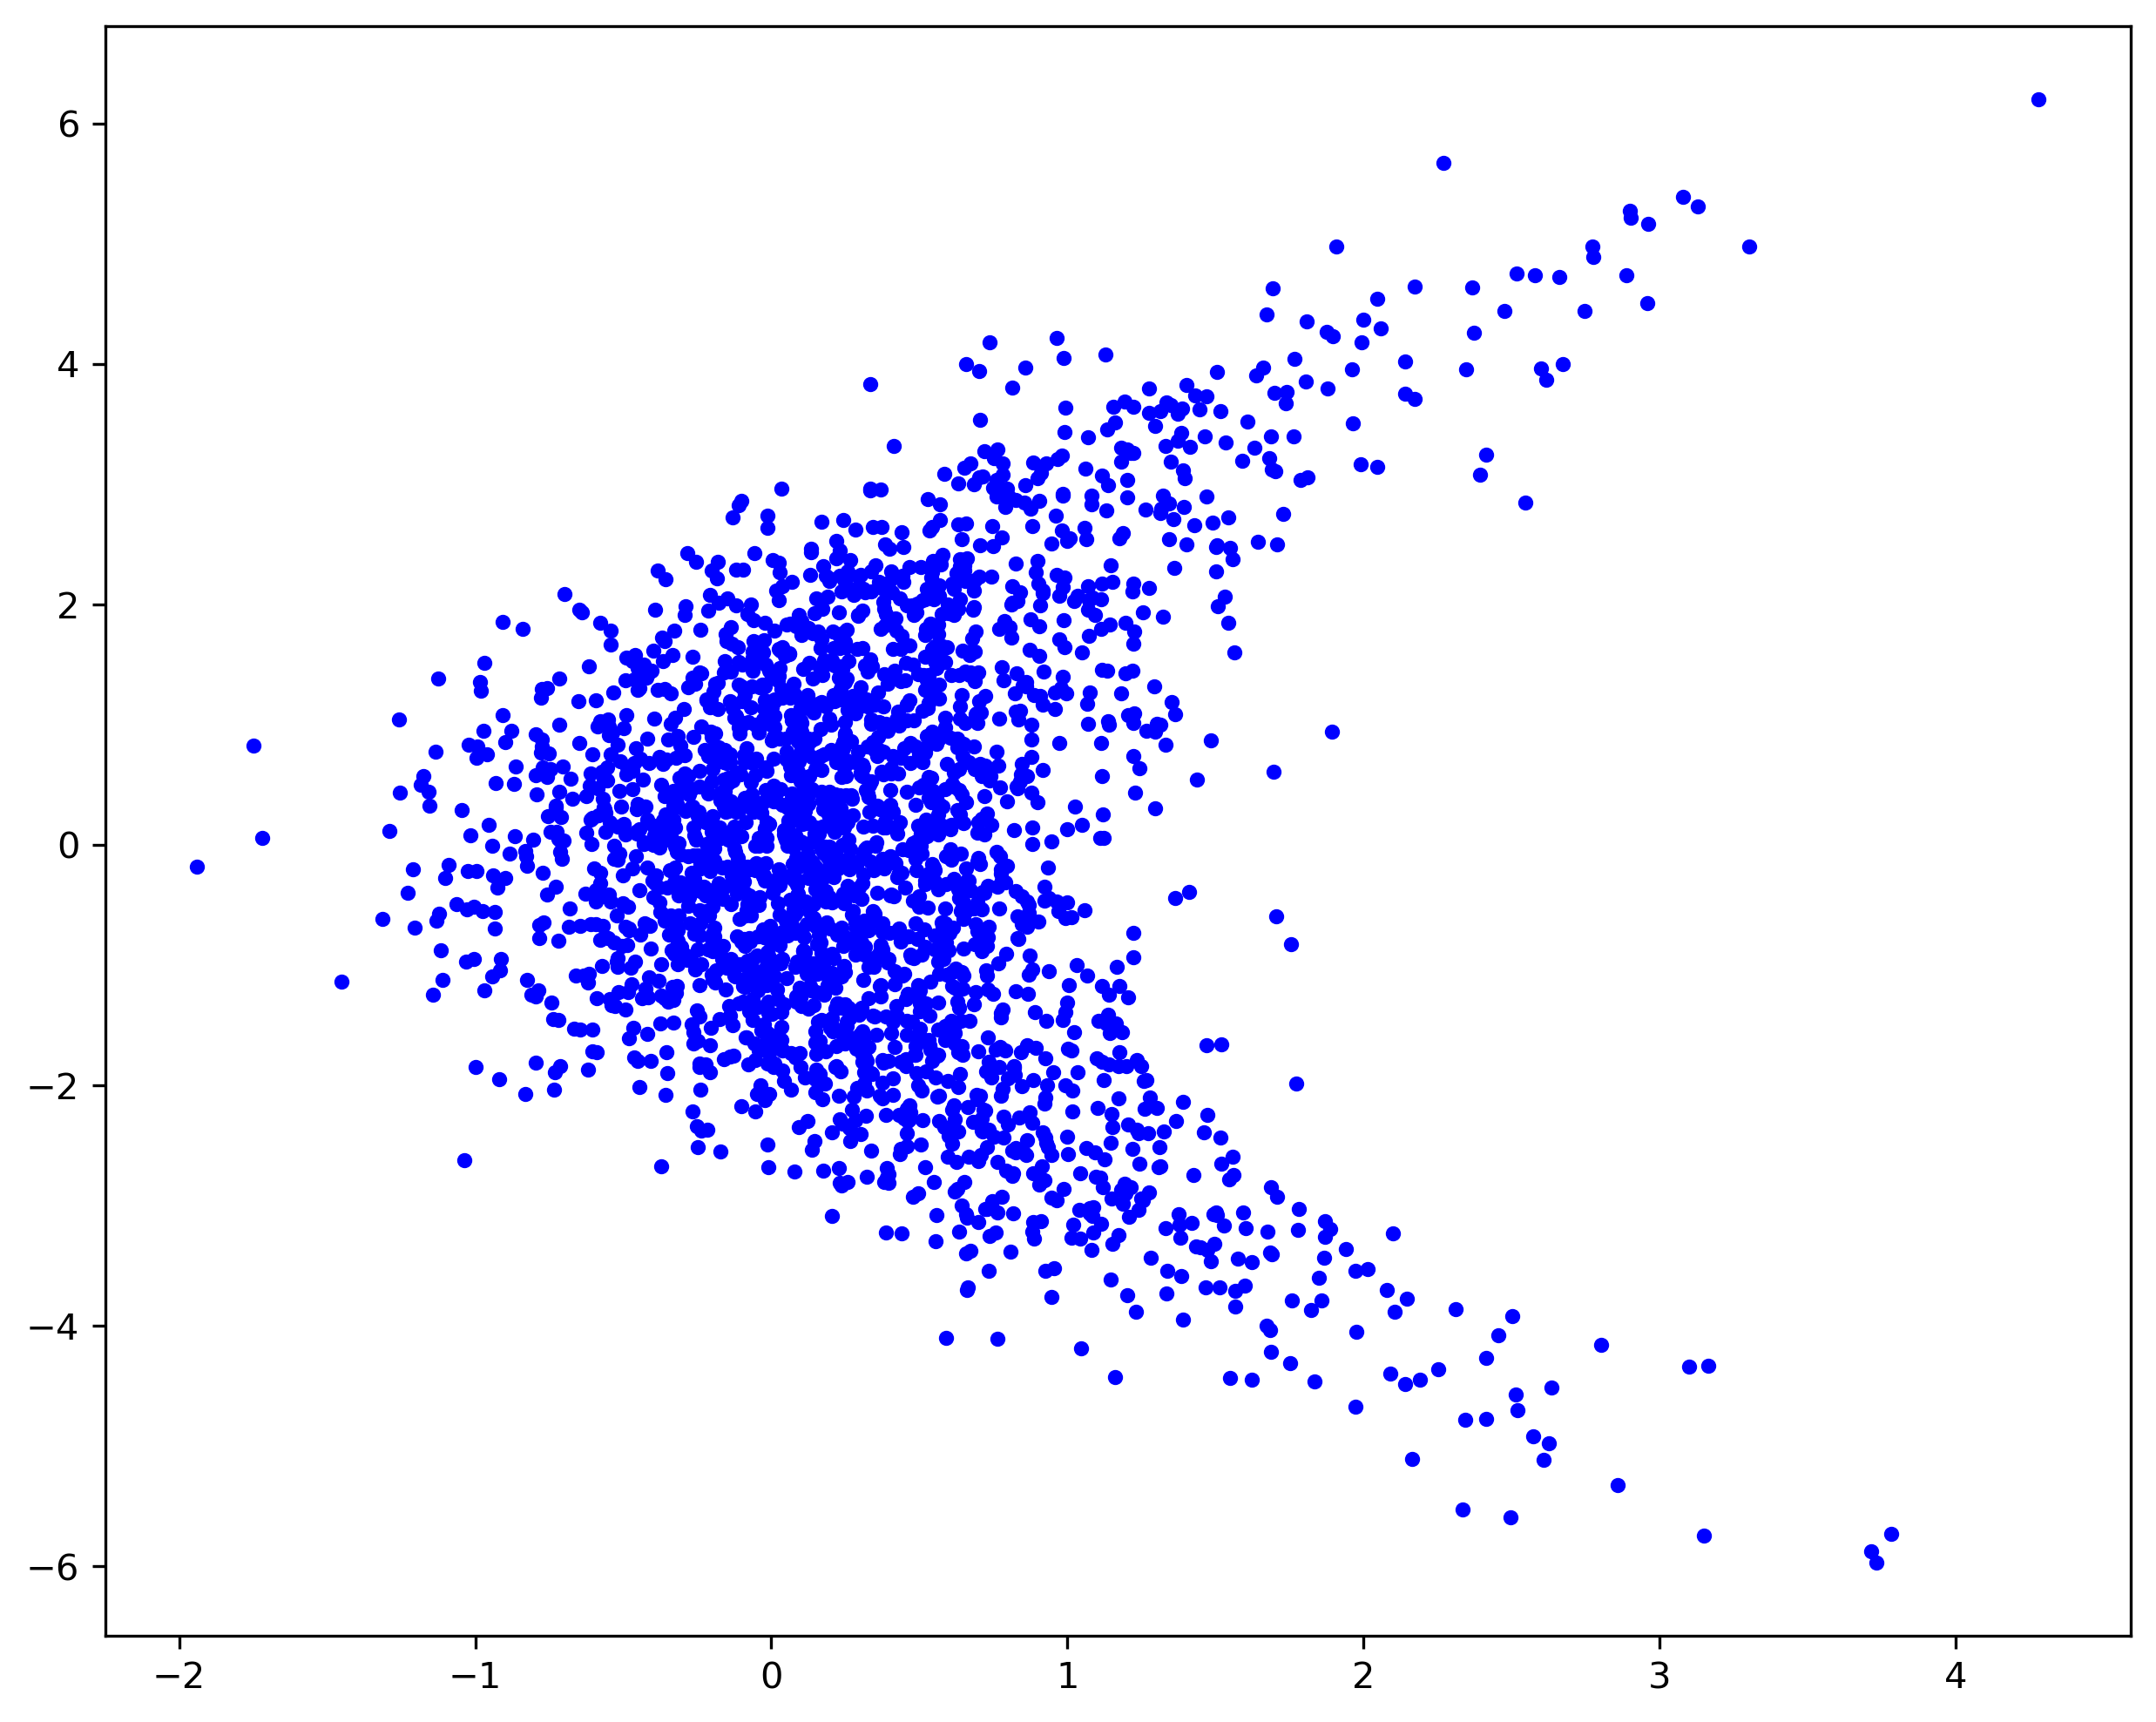
\includegraphics[width=\textwidth]{Chapter5/results/visualisations/datasets/single_banana.png}
\caption{Single Banana}
\end{subfigure}
\begin{subfigure}[b]{0.32\textwidth}
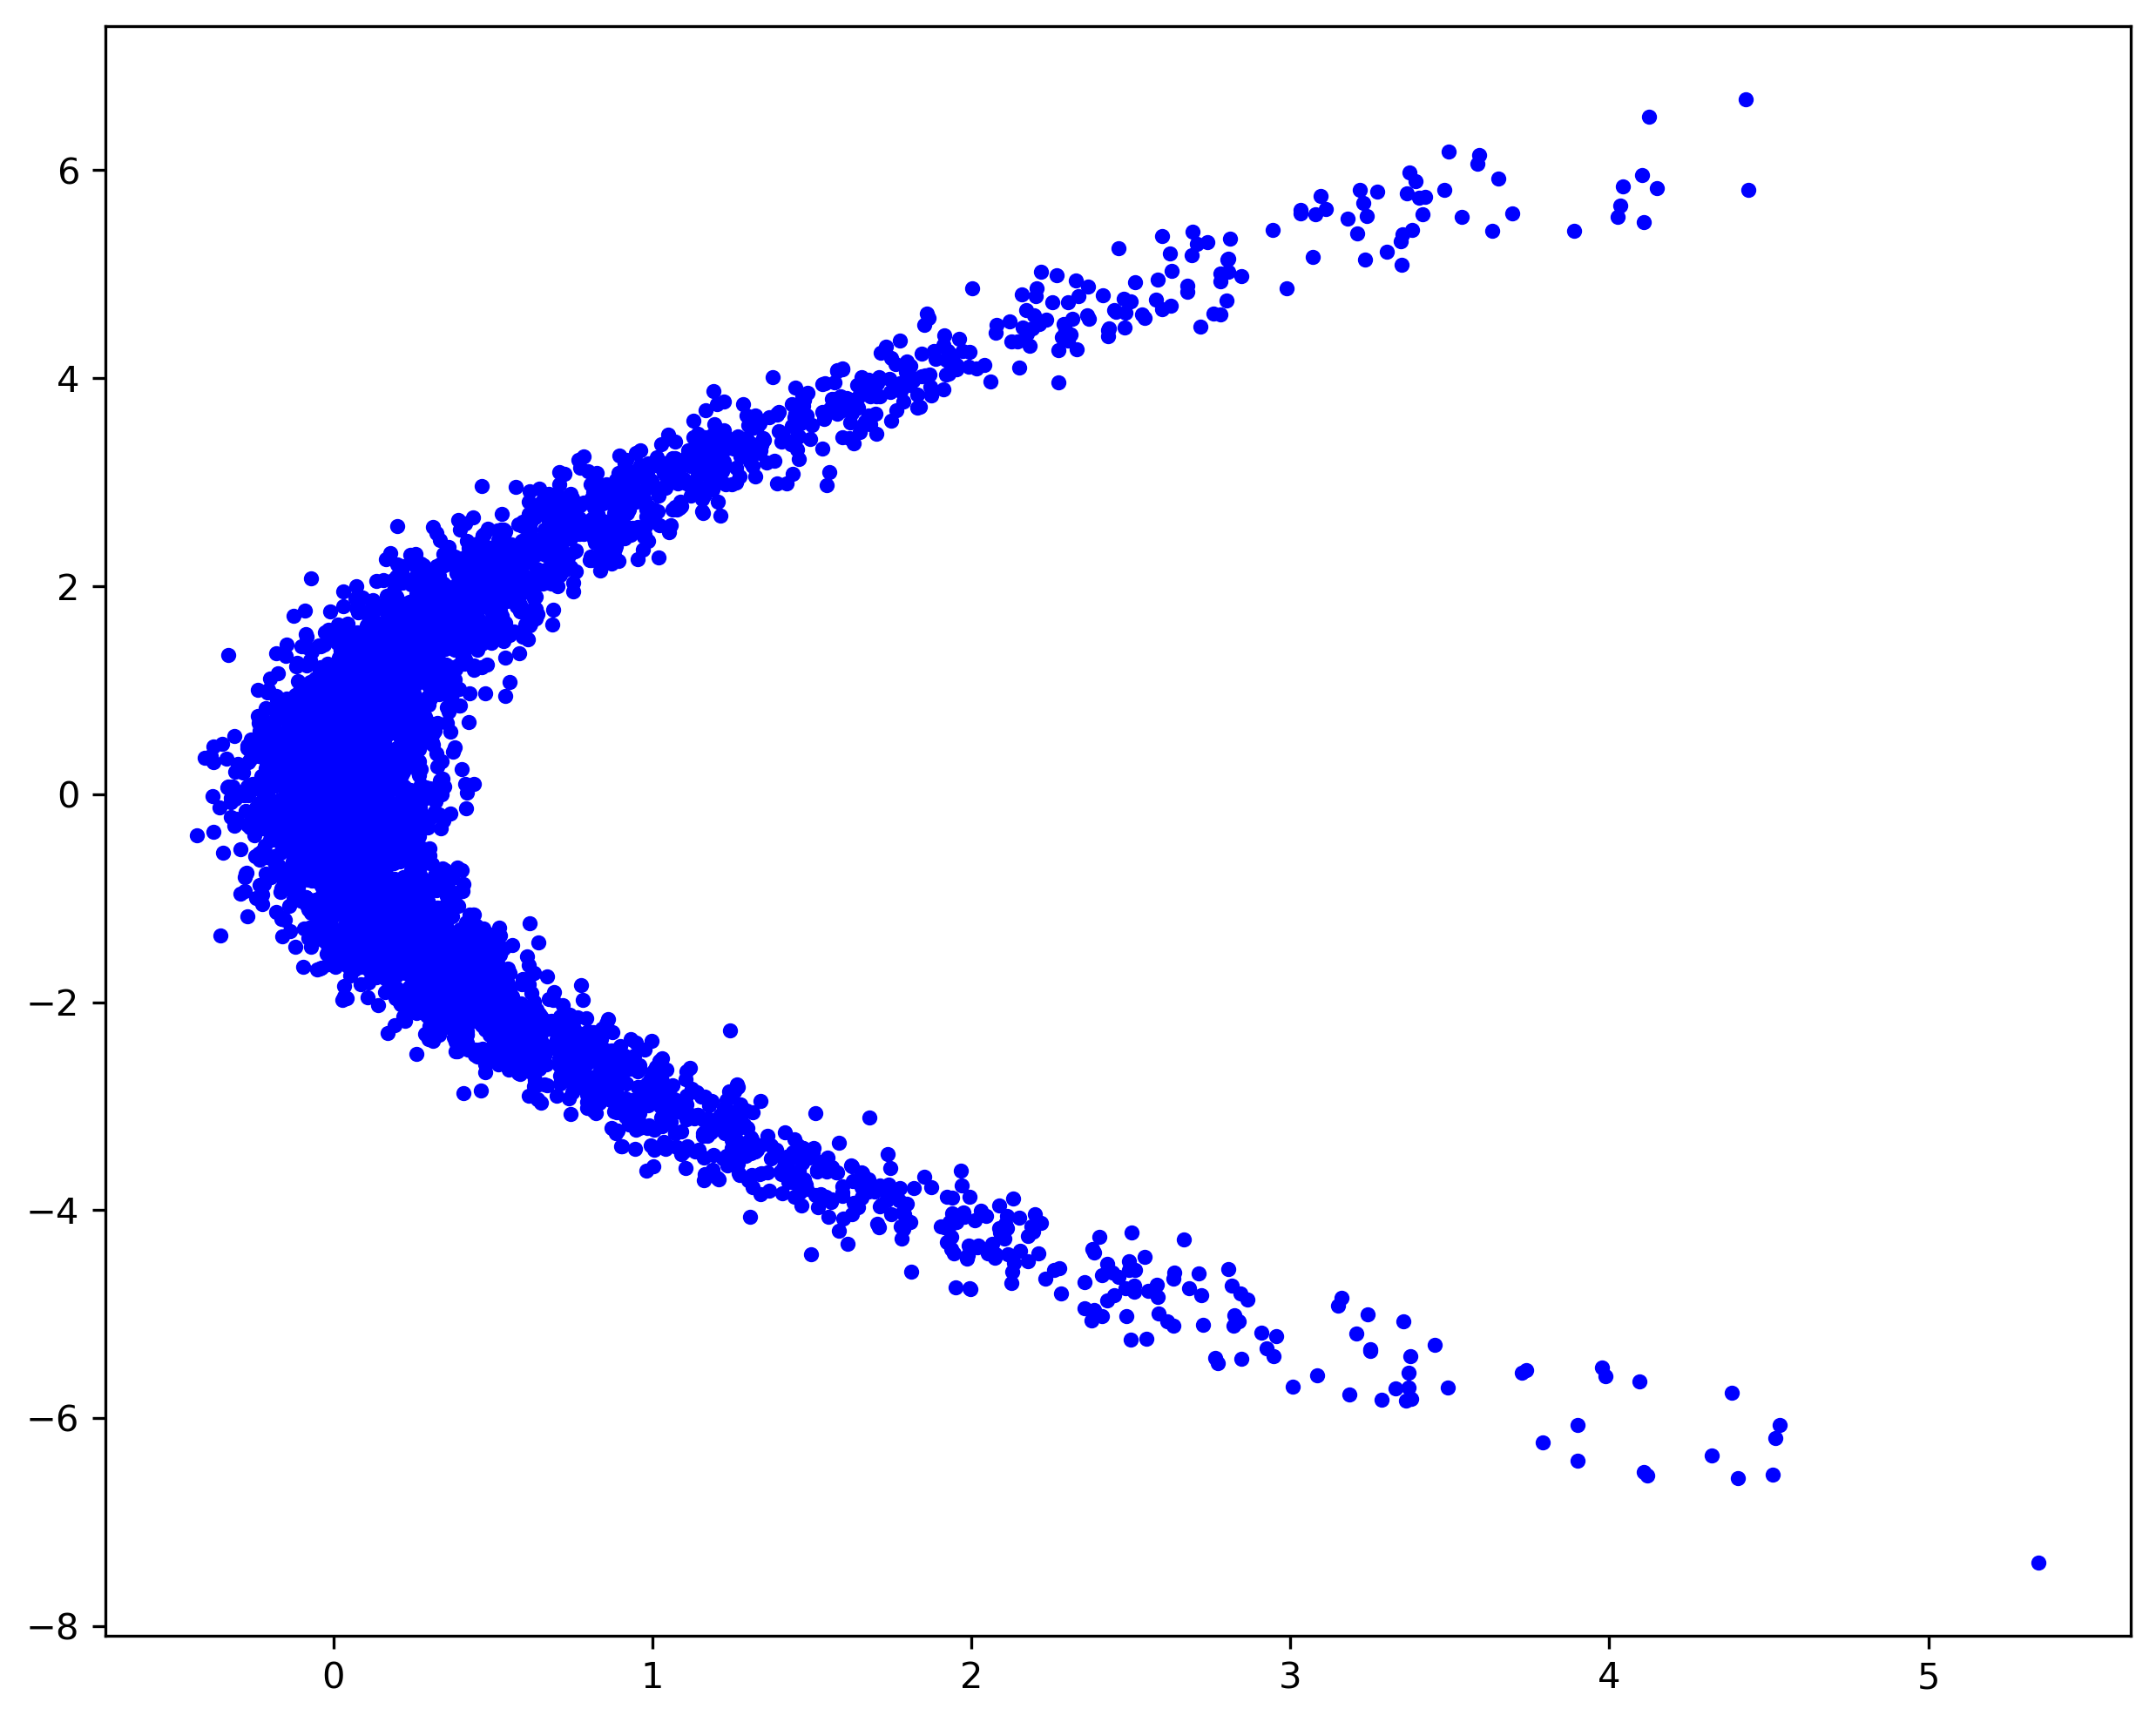
\includegraphics[width=\textwidth]{Chapter5/results/visualisations/datasets/squeezed_single_banana.png}
\caption{Squeezed Single Banana}
\end{subfigure}
\begin{subfigure}[b]{0.32\textwidth}
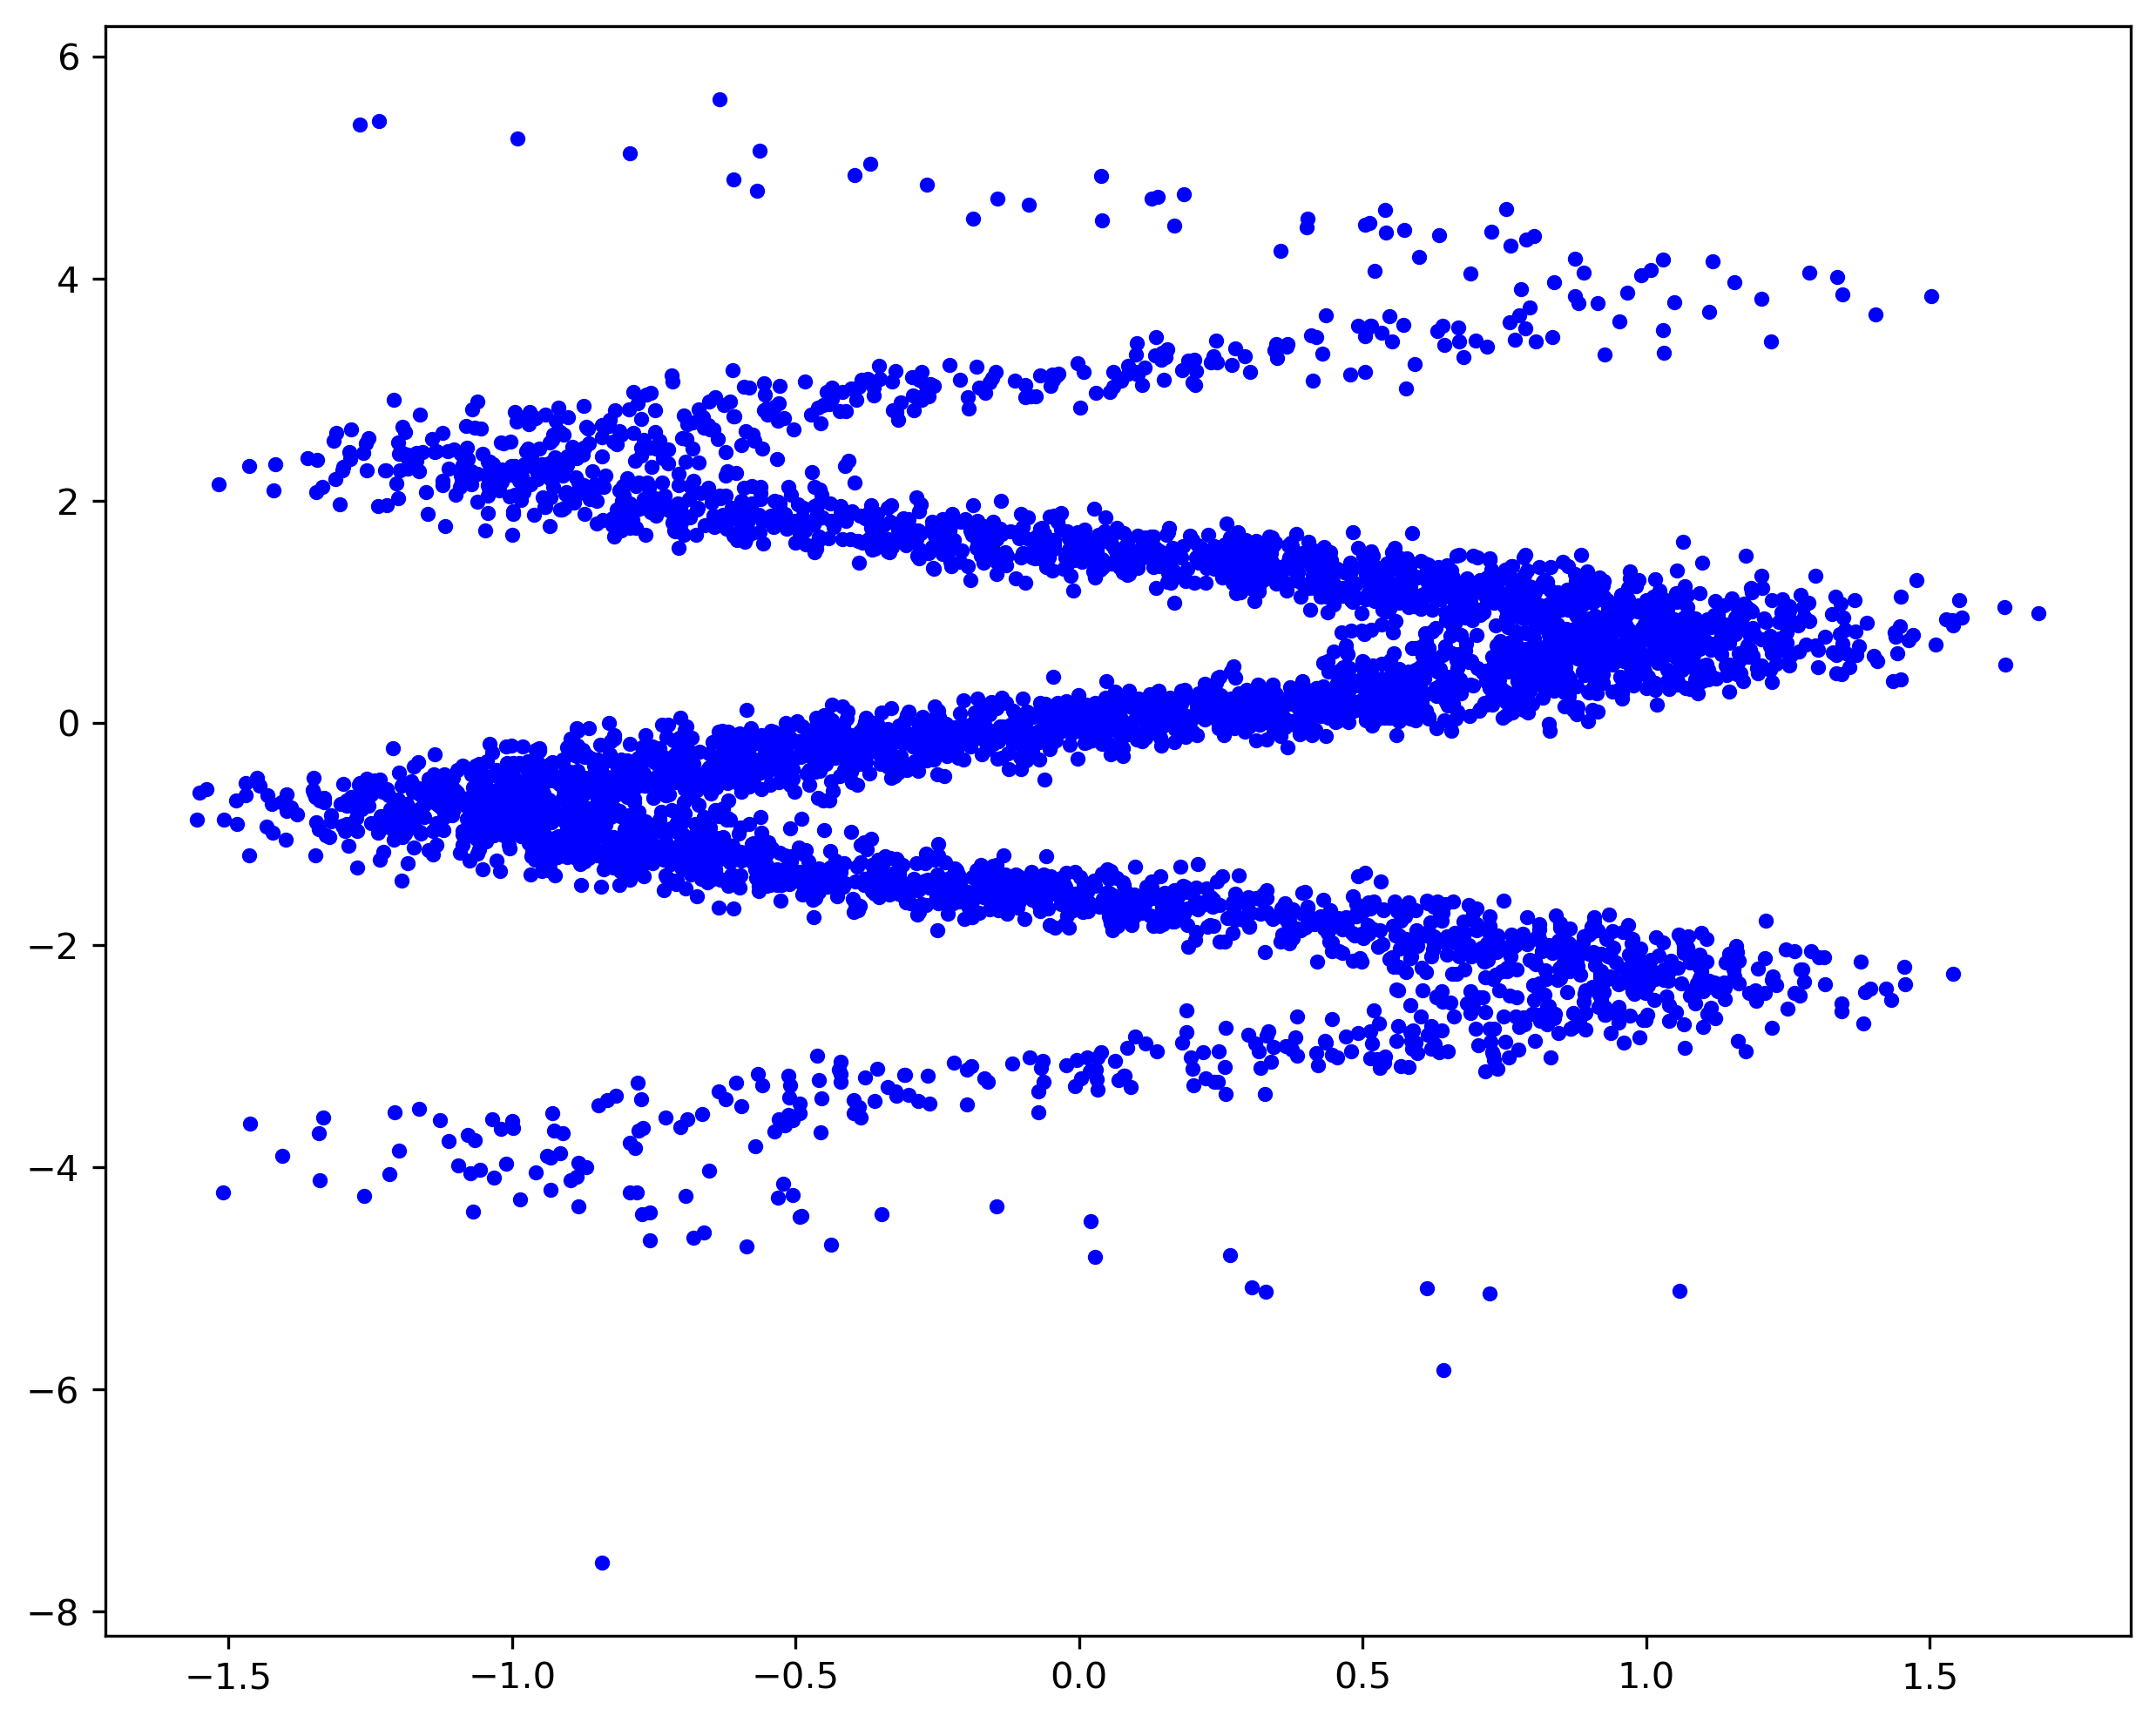
\includegraphics[width=\textwidth]{Chapter5/results/visualisations/datasets/river.png}
\caption{River}
\end{subfigure}
\caption{Visualization of the datasets used in our manifold mapping experiments.}
\label{fig:datasets}
\end{figure}

In our manifold mapping experiments (see Section~\ref{sec:manifold-mappings-experiments}), we use the following datasets illustrated in Figure~\ref{fig:datasets}:

\begin{itemize}
    \item \textit{Single Banana Dataset}: A two-dimensional dataset shaped like a curved banana.
    \item \textit{Squeezed Single Banana Dataset}: A variant of the Single Banana with a tighter bend.
    \item \textit{River Dataset}: A more complex 2D dataset resembling the meandering path of a river.
\end{itemize}

Each dataset is constructed by defining specific diffeomorphisms $\diffeo$ and convex quadratic functions $\psi$, then sampling from the resulting probability density using Langevin Monte Carlo Markov Chain (MCMC) with Metropolis-Hastings correction. The probability density function is defined as:

\begin{equation}
    p(\mathbf{x}) \propto e^{-\psi(\diffeo(\mathbf{x}))},
    \label{eq:stroco-diffeo-density-ap}
\end{equation}

\noindent where the strongly convex function $\psi$ is given by:

\begin{equation}
    \psi(\mathbf{x}) = \frac{1}{2} \mathbf{x}^\top \mathbf{A}^{-1} \mathbf{x},
    \label{eq:quadratic-stroco-ap}
\end{equation}

\noindent and $\mathbf{A}$ is a positive-definite diagonal matrix. The specific choices of $\diffeo$ and $\mathbf{A}$ for each dataset determine its geometric properties.

\subsubsection{Diffeomorphisms and Convex Quadratic Functions}

The key differences between the datasets arise from the diffeomorphism $\diffeo$ and the covariance matrix $\mathbf{A}$ used in the sampling process. Below, we describe the specific settings for each dataset.

\paragraph{1. Single Banana Dataset}

\begin{itemize}
    \item Diffeomorphism: 
    \[
    \diffeo(\mathbf{x}) = \begin{pmatrix} 
    x_1 - a x_2^2 - z \\
    x_2 
    \end{pmatrix}
    \]
    where $a = \frac{1}{9}$ and $z = 0$.
    \item Covariance matrix:
    \[
    \mathbf{A} = \begin{pmatrix} 
    \frac{1}{4} & 0 \\
    0 & 4 
    \end{pmatrix}
    \]
\end{itemize}

\paragraph{2. Squeezed Single Banana Dataset}

\begin{itemize}
    \item Diffeomorphism: Same as the Single Banana Dataset.
    \item Covariance matrix:
    \[
    \mathbf{A} = \begin{pmatrix} 
    \frac{1}{81} & 0 \\
    0 & 4 
    \end{pmatrix}
    \]
\end{itemize}

\paragraph{3. River Dataset}

\begin{itemize}
    \item Diffeomorphism: 
    \[
    \diffeo(\mathbf{x}) = \begin{pmatrix} 
    x_1 - \sin(a x_2) - z \\
    x_2 
    \end{pmatrix}
    \]
    where $a = 2$ and $z = 0$.
    \item Covariance matrix:
    \[
    \mathbf{A} = \begin{pmatrix} 
    \frac{1}{25} & 0 \\
    0 & 3 
    \end{pmatrix}
    \]
\end{itemize}

\subsubsection{Dataset Generation Algorithm}

Algorithm~\ref{alg:Langevin-MCMC-with-M-H-correction} outlines the dataset generation process for all three datasets. The specific diffeomorphisms and quadratic functions differ for each dataset.

\begin{algorithm}[h]
\caption{General Dataset Generation Algorithm}
\label{alg:Langevin-MCMC-with-M-H-correction}
\begin{algorithmic}[1]
\REQUIRE Number of samples $N$, MCMC steps $T$, Step size $\delta$, Diffeomorphism $\diffeo$, Covariance matrix $\mathbf{\Lambda}$
\ENSURE Dataset $\{\mathbf{x}_1, \mathbf{x}_2, \dots, \mathbf{x}_N\}$
\STATE Initialize: Set initial state $\mathbf{x}_0 = \mathbf{0} \in \mathbb{R}^2$.
\FOR{$i = 1$ to $N$}
    \STATE $\mathbf{x} = \mathbf{x}_0$
    \FOR{$k = 1$ to $T$}
        \STATE Compute the score function $\nabla_{\mathbf{x}} \log p_{\text{target}}(\mathbf{x})$.
        \STATE Propose $\mathbf{x}' = \mathbf{x} + \frac{\delta^2}{2} \nabla_{\mathbf{x}} \log p_{\text{target}}(\mathbf{x}) + \delta \boldsymbol{\eta}$, where $\boldsymbol{\eta} \sim \mathcal{N}(\mathbf{0}, \mathbf{I}_2)$.
        
        \STATE Compute the forward kernel:
        \[
        K_{\text{forward}} = \frac{|\mathbf{x} - \mathbf{x}' + \frac{\delta^2}{2} \nabla_{\mathbf{x}'} \log p_{\text{target}}(\mathbf{x}')|^2}{2\delta^2}
        \]

        \STATE Compute the reverse kernel:
        \[
        K_{\text{reverse}} = \frac{|\mathbf{x}' - \mathbf{x} + \frac{\delta^2}{2} \nabla_{\mathbf{x}} \log p_{\text{target}}(\mathbf{x})|^2}{2\delta^2}
        \]
        
        \STATE Compute the Metropolis-Hastings acceptance probability:
        \[
        A = \min\left(1, \frac{p_{\text{target}}(\mathbf{x}')}{p_{\text{target}}(\mathbf{x})} \exp\left( -K_{\text{forward}} + K_{\text{reverse}} \right) \right)
        \]
        
        \STATE Accept $\mathbf{x}'$ with probability $A$; else set $\mathbf{x}' = \mathbf{x}$.
        \STATE Update $\mathbf{x} = \mathbf{x}'$.
    \ENDFOR
    \STATE Store the final $\mathbf{x}$ as sample $\mathbf{x}_i$.
\ENDFOR
\end{algorithmic}
\end{algorithm}

\subsection{Datasets for Riemannian Autoencoder Experiments}
\label{app:rae_datasets}

In the Riemannian autoencoder experiments (see Section~\ref{sec:RAE-experiments}), we use the following datasets:
\begin{itemize}
    \item \textit{Hemisphere}(\textit{d'}, \textit{d}) Dataset: Samples drawn from the upper hemisphere of a \textit{d'}-dimensional unit sphere and embedded into $\mathbb{R}^d$ via a random isometric mapping.
    \item \textit{Sinusoid}(\textit{d'}, \textit{d}) Dataset: Generated by applying sinusoidal transformations to \textit{d'}-dimensional latent variables, resulting in a complex, nonlinear manifold in $\mathbb{R}^d$.
\end{itemize}

\subsection{\texorpdfstring{Hemisphere($d'$, $d$)}{Hemisphere(d', d)} Dataset}

The \textit{Hemisphere}($d'$, $d$) dataset consists of samples drawn from the upper hemisphere of a $d'$-dimensional unit sphere, which are then embedded into a $d$-dimensional ambient space using a random isometric embedding. Below are the steps involved in constructing this dataset.

\paragraph{1. Sampling from the Upper Hemisphere}

We begin by sampling points from the upper hemisphere of the $d'$-dimensional unit sphere $S^{d'}_+ \subset \mathbb{R}^{d'+1}$. The upper hemisphere is defined as:
\[
S^{d'}_+ = \left\{ \mathbf{x} \in \mathbb{R}^{d'+1} : \|\mathbf{x}\| = 1, \, x_1 \geq 0 \right\}.
\]
The first angular coordinate $\theta_1$ is sampled from a Beta distribution with shape parameters $\alpha = 5$ and $\beta = 5$, scaled to the interval $\left[ 0, \frac{\pi}{2} \right]$. This sampling method emphasizes points near the ``equator'' of the hemisphere. The remaining angular coordinates $\theta_2, \ldots, \theta_{d'}$ are sampled uniformly from the interval $\left[ 0, \pi \right]$:
\[
\theta_1 \sim \text{Beta}(5, 5) \cdot \left( \frac{\pi}{2} \right), \quad \theta_i \sim \text{Uniform}(0, \pi), \, \text{for } i = 2, \ldots, d'.
\]

\paragraph{2. Conversion to Cartesian Coordinates}

Next, each sampled point in spherical coordinates is converted into Cartesian coordinates in $\mathbb{R}^{d'+1}$ using the following transformation equations:
\[
x_1 = \cos(\theta_1), \quad x_2 = \sin(\theta_1) \cos(\theta_2), \quad \dots, \quad x_{d'+1} = \sin(\theta_1) \sin(\theta_2) \cdots \sin(\theta_{d'}).
\]
This conversion ensures that the sampled points lie on the surface of the unit sphere in $(d'+1)$-dimensional space.

\paragraph{3. Random Isometric Embedding into $\mathbb{R}^d$}

After sampling points on the hemisphere in $\mathbb{R}^{d'+1}$, the points are embedded into a $d$-dimensional ambient space ($d \geq d'+1$) using a random isometric embedding. The embedding process is as follows:

\begin{enumerate}
    \item Generate a random matrix $\mathbf{A} \in \mathbb{R}^{d \times (d'+1)}$, where each entry is sampled from a standard normal distribution $\mathcal{N}(0, 1)$.
    \item Perform a QR decomposition on matrix $\mathbf{A}$ to obtain $\mathbf{Q} \in \mathbb{R}^{d \times (d'+1)}$:
    \[
    \mathbf{A} = \mathbf{Q} \mathbf{R}.
    \]
    The columns of \( \mathbf{Q} \) form an orthonormal basis for a \((d'+1)\)-dimensional subspace of \( \mathbb{R}^d \), ensuring that \( \mathbf{Q} \) defines an isometric embedding from \( \mathbb{R}^{d'+1} \) into \( \mathbb{R}^d \). This guarantees that distances and angles are preserved during the mapping, maintaining the geometric structure of the original space within the higher-dimensional ambient space.

    \item Use matrix $\mathbf{Q}$ to map each sample $\mathbf{x} \in \mathbb{R}^{d'+1}$ into the ambient space:
    \[
    \mathbf{y} = \mathbf{Q}\mathbf{x},
    \]
    where $\mathbf{y} \in \mathbb{R}^d$ are the embedded samples.
\end{enumerate}

\begin{algorithm}[H]
    \caption{Hemisphere($d'$, $d$) Dataset Generation}
    \begin{algorithmic}[1]
        \STATE \textbf{Input:} Intrinsic dimension $d'$, ambient dimension $d$, number of samples $n$, Beta distribution parameters $\alpha = 5$, $\beta = 5$
        \STATE \textbf{Output:} Dataset $\mathbf{Y} \in \mathbb{R}^{n \times d}$

        \STATE \textbf{Step 1: Generate Random Isometric Embedding}
        \STATE Generate a random matrix $\mathbf{A} \in \mathbb{R}^{d \times (d'+1)}$ with entries from $\mathcal{N}(0, 1)$
        \STATE Perform QR decomposition on $\mathbf{A}$ to obtain $\mathbf{Q} \in \mathbb{R}^{d \times (d'+1)}$:
        \[
        \mathbf{A} = \mathbf{Q} \mathbf{R}
        \]

        \STATE \textbf{Step 2: Construct Dataset}
        \FOR{$i = 1$ to $n$}
            \STATE \textbf{Step 2.1: Sample Spherical Coordinates}
            \STATE Sample the first angular coordinate $\theta_1$ from a scaled Beta distribution:
            \[
            \theta_1 \sim \text{Beta}(\alpha, \beta) \cdot \left( \frac{\pi}{2} \right)
            \]
            \STATE Sample the remaining angular coordinates $\theta_2, \dots, \theta_{d'}$ from a uniform distribution:
            \[
            \theta_i \sim \text{Uniform}(0, \pi), \quad \text{for } i = 2, \dots, d'
            \]

            \STATE \textbf{Step 2.2: Convert to Cartesian Coordinates}
            \STATE Convert the spherical coordinates to Cartesian coordinates $\mathbf{x}_i \in \mathbb{R}^{d'+1}$ using:
            \[
            x_1 = \cos(\theta_1), \quad x_2 = \sin(\theta_1) \cos(\theta_2), \dots, \quad x_{d'+1} = \sin(\theta_1) \sin(\theta_2) \cdots \sin(\theta_{d'}).
            \]

            \STATE \textbf{Step 2.3: Embed Sample $\mathbf{x}_i$ into Ambient Space}
            \STATE Map the sample $\mathbf{x}_i$ to the ambient space using:
            \[
            \mathbf{y}_i = \mathbf{Q} \mathbf{x}_i
            \]

            \STATE Append $\mathbf{y}_i$ to the dataset $\mathbf{Y}$
        \ENDFOR
        
        \STATE \textbf{Return:} The final dataset $\mathbf{Y} = [\mathbf{y}_1, \mathbf{y}_2, \dots, \mathbf{y}_n]$
    \end{algorithmic}
\end{algorithm}

\subsection{\texorpdfstring{Sinusoid($d'$, $d$)}{Sinusoid(d', d)} Dataset}

The \textit{Sinusoid}($d'$, $d$) dataset represents a $d'$-dimensional manifold embedded in $d$-dimensional space through nonlinear sinusoidal transformations. Below are the detailed steps involved in constructing this dataset.

\paragraph{1. Sampling Latent Variables}

The latent variables $\mathbf{z} \in \mathbb{R}^{d'}$ are sampled from a multivariate Gaussian distribution with zero mean and isotropic variance, as follows:
\[
\mathbf{z} \sim \mathcal{N}\left( 0, \sigma_m^2 I_{d'} \right),
\]
where $\sigma_m^2$ controls the variance along each intrinsic dimension, and $I_{d'}$ is the $d' \times d'$ identity matrix. The value of $\sigma_m^2$ is set to 3 for our experiments.

\paragraph{2. Defining Ambient Coordinates with Sinusoidal Transformations}

For each of the $d-d'$ ambient dimensions, we construct a shear vector \( \mathbf{a}_j \in \mathbb{R}^{d'} \), with its elements drawn uniformly from the interval \([1, 2]\):
\[
\mathbf{a}_j \sim \text{Uniform}(1, 2)^{d'}, \quad \text{for } j = 1, \dots, d-d'.
\]

The shear vectors \( \mathbf{a}_j \) apply a fixed linear transformation to the latent space \( \mathbf{z} \in \mathbb{R}^{d'} \), determining how the latent variables influence each ambient dimension. These vectors, sampled once for each of the $d-d'$ ambient dimensions, modulate the scale and periodicity of the sinusoidal transformation.

Each ambient coordinate \( x_j \) is generated as a sinusoidal function of the inner product between \( \mathbf{a}_j \) and \( \mathbf{z} \), with a small Gaussian noise added for regularization.

\[
x_j = \sin\left( \mathbf{a}_j^\top \mathbf{z} \right) + \epsilon_j,
\]
where \( \epsilon_j \sim \mathcal{N}(0, \sigma_a^2) \) is Gaussian noise with variance \( \sigma_a^2 \). In our experiments, we set \( \sigma_a^2 = 10^{-3} \).

\paragraph{3. Constructing the Dataset Samples}

The final samples $\mathbf{y} \in \mathbb{R}^d$ are formed by concatenating the ambient coordinates $x_1, x_2, \dots, x_{d-d'}$ with the latent variables $z_1, z_2, \dots, z_{d'}$:
\[
\mathbf{y} = \left[ x_1, x_2, \dots, x_{d-d'}, \, z_1, z_2, \dots, z_{d'} \right]^\top.
\]

\begin{algorithm}[H]
    \caption{Sinusoid($d'$, $d$) Dataset Generation}
    \begin{algorithmic}[1]
        \STATE \textbf{Input:} Intrinsic dimension $d'$, ambient dimension $d$, number of samples $n$, variance $\sigma_m^2 = 3$, noise variance $\sigma_a^2 = 10^{-3}$
        \STATE \textbf{Output:} Dataset $\mathbf{Y} \in \mathbb{R}^{n \times d}$

        \STATE \textbf{Step 1: Generate Shear Vectors}
        \FOR{$j = 1$ to $d - d'$}
            \STATE Sample shear vector $\mathbf{a}_j \in \mathbb{R}^{d'}$ from \text{Uniform}$(1, 2)^{d'}$
        \ENDFOR

        \STATE \textbf{Step 2: Construct Dataset}
        \FOR{$i = 1$ to $n$}
            \STATE \textbf{Step 2.1: Sample Latent Variables}
            \STATE Generate latent variables $\mathbf{z}_i \in \mathbb{R}^{d'}$ from a multivariate Gaussian:
            \[
            \mathbf{z}_i \sim \mathcal{N}(0, \sigma_m^2 \cdot I_{d'})
            \]

            \STATE \textbf{Step 2.2: Compute Ambient Coordinates for Sample $i$}
            \FOR{$j = 1$ to $d - d'$}
                \STATE Compute ambient coordinate $x_j$ for the $i$-th sample:
                \[
                x_j = \sin\left( \mathbf{a}_j^\top \mathbf{z}_i \right) + \epsilon_j, \quad \epsilon_j \sim \mathcal{N}(0, \sigma_a^2)
                \]
            \ENDFOR

            \STATE \textbf{Step 2.3: Form Final Sample $\mathbf{y}_i$}
            \STATE Concatenate the ambient coordinates $\mathbf{x} = [x_1, x_2, \dots, x_{d-d'}]$ and the latent variables $\mathbf{z}_i$ to form the final sample $\mathbf{y}_i \in \mathbb{R}^d$:
            \[
            \mathbf{y}_i = [x_1, x_2, \dots, x_{d-d'}, z_1, z_2, \dots, z_{d'}]^\top
            \]

            \STATE Append $\mathbf{y}_i$ to the dataset $\mathbf{Y}$
        \ENDFOR
        
        \STATE \textbf{Return:} The final dataset $\mathbf{Y} = [\mathbf{y}_1, \mathbf{y}_2, \dots, \mathbf{y}_n]$
    \end{algorithmic}
\end{algorithm}

\subsection{Gaussian Blobs Image Manifold}

The \textit{Gaussian Blobs Image Manifold} dataset defines an image manifold with a controllable intrinsic dimension $d'$ (number of Gaussian blobs) embedded in a 1024-dimensional ambient space (32 × 32 pixel images). The dataset is constructed as follows:
\begin{enumerate}
    \item $d'$ Gaussian blob centers are randomly selected from a 32 × 32 grid without replacement. These centers are fixed and remain the same for all points in the dataset.
    \item For each image, a Gaussian mixture is generated by centering Gaussian distributions at the fixed locations, with standard deviations sampled uniformly from a specified range $[s_{\min}, s_{\max}]$.
    \item The normalized density of the Gaussian mixture defines the intensity values of the 2D image. Each combination of standard deviations uniquely defines a point on the manifold.
\end{enumerate}

\begin{algorithm}[h]
\caption{Gaussian Blobs Image Manifold Dataset Generation}
\label{alg:gaussian_blobs}
\begin{algorithmic}[1]
\REQUIRE Number of samples $N$, intrinsic dimension $d'$, image size $I$, standard deviation range $[s_{\min}, s_{\max}]$, random seed $S$
\ENSURE Dataset $\{\mathbf{x}_1, \mathbf{x}_2, \dots, \mathbf{x}_N\}$ with $\mathbf{x}_i \in \mathbb{R}^{I \times I}$
\STATE Initialize: Set random seed $S$ for reproducibility.
\STATE Generate $d'$ Gaussian centers by sampling without replacement from the $I \times I$ pixel grid. \textbf{These centers are fixed for all samples in the dataset.}
\FOR{$i = 1$ to $N$}
    \STATE Initialize an empty image $\mathbf{x}_i$ of size $I \times I$.
    \FOR{$j = 1$ to $d'$}
        \STATE Select the $j$-th Gaussian center $(x_j, y_j)$ from the preselected centers.
        \STATE Sample standard deviation $s_j$ uniformly from $[s_{\min}, s_{\max}]$.
        \STATE Compute the Gaussian density over the entire image grid:
        \[
        g(x, y) = \frac{1}{\sqrt{2 \pi} s_j} \exp\left(-\frac{(x - x_j)^2 + (y - y_j)^2}{2 s_j^2}\right)
        \]
        \STATE Add the Gaussian density to the image: $\mathbf{x}_i(x, y) \mathrel{+}= g(x, y)$.
    \ENDFOR
    \STATE Normalize $\mathbf{x}_i$ to the range $[0, 1]$:
    \[
    \mathbf{x}_i = \frac{\mathbf{x}_i - \min(\mathbf{x}_i)}{\max(\mathbf{x}_i) - \min(\mathbf{x}_i)}
    \]
    \STATE Store the normalized image $\mathbf{x}_i$ as a sample.
\ENDFOR
\end{algorithmic}
\end{algorithm}

\section{Data Manifold Approximation}
\label{app:data_manifold_approximation}

The learned manifold, shown in orange in Figure~\ref{fig:learned_charts}, corresponds to the set $D_{\epsilon}(\mathcal{U})$, where $D_{\epsilon}$ denotes the RAE decoder defined in Eq.~\ref{eq:rae-decoder}, the set \( \mathcal{U} \) in the latent space is the open set given by
% Mathematically, let \( \manifold \subset \mathbb{R}^\dimInd \) represent the manifold embedded in the ambient space, and let \( \mathcal{U} \) be an open subset of \( \mathbb{R}^{d_{\epsilon}} \), defined as:
\[
    \mathcal{U} = \prod_{i=1}^{d_{\epsilon}} (-3\sqrt{\spdMatrixDiag_{\coordIndA_\sumIndA}}, 3\sqrt{\spdMatrixDiag_{\coordIndA_\sumIndA}})
\]
and \( \spdMatrixDiag_{\coordIndA_1}, \dots, \spdMatrixDiag_{\coordIndA_{d_{\epsilon}}} \) are the \( d_{\epsilon} \) highest learned variances corresponding to the ones used in the RAE construction. 

To visualize this in practice, we construct a mesh grid by linearly sampling each latent dimension from \( -3\sqrt{\spdMatrixDiag_{\coordIndA_\sumIndA}} \) to \( +3\sqrt{\spdMatrixDiag_{\coordIndA_\sumIndA}} \), for \( i = 1, \dots, d_{\epsilon} \), where \( d_{\epsilon} \) is the number of significant latent dimensions. Practically, the off-manifold latent dimensions (those corresponding to negligible variances) are set to zero. The decoder \( D_{\epsilon} \) then maps this grid from \( \mathcal{U} \) back to \( \mathbb{R}^\dimInd \), generating an approximation of the data manifold, as illustrated in Figure~\ref{fig:learned_charts}.

\section{Explanation for the Need of Higher Regularity in Non-Affine Flows}
\label{app:expanded_loss_function}

As described in Section~\ref{sec:image_datasets}, introducing a small regularization term involving the Hessian vector product of the flow can substantially improve the RAE’s ability to assign higher variances to the on-manifold (semantically meaningful) directions and suppress variances in off-manifold directions for \textit{non-affine} flows. The core issue arises from the fact that, for \emph{non-affine} normalizing flows, the second-order derivatives of \(\diffeo_{\networkParams_2}\) appear in the Hessian of the modeled log-density in a way that can adversely impact the performance of the RAE if left unregularized, as we shall see below.

\subsection{Hessian of the Log-Density and Intrinsic Dimensionality}
Recently, Stanczuk et al.~\cite{pmlr-v235-stanczuk24a} formally proved—and Stanczuk and Batzolis et al.~\cite{pmlr-v235-stanczuk24a}, as well as Wenliang and Moran~\cite{wenliang2022score}, independently discovered and demonstrated empirically—that when data are locally concentrated around a lower-dimensional manifold of intrinsic dimension \(k\), the \textit{Jacobian} of the score function or equivalently, the \textit{Hessian} of the log-density has \(k\) vanishing singular values. The eigenvectors corresponding to these vanishing singular values span the local tangent space of the data manifold. Consequently, for a trained model, large singular values of \(\nabla_{\mathbf{x}}^2\!\log p_{\theta_1, \theta_2}(\mathbf{x})\) indicate \emph{off-manifold} directions, while near-zero singular values reveal \emph{on-manifold} directions—those spanning the locally flat subspace in which the data reside.

\subsection{Analyzing the Hessian of the Log-Density of Our Model}
With the background knowledge on the connection between the Hessian of the log-density and the local intrinsic structure in mind, let's investigate the Hessian of the logdensity of our model under the assumption that $\diffeo_{\networkParams_2}$ is local isometry and hence volume preserving as well. The modeled density function is
\begin{equation}
\label{eq:app_flow_density}
    p_{\theta_1, \theta_2}(\mathbf{x})
    \;=\;
    p_{\theta_1}\bigl(\diffeo_{\networkParams_2}(\mathbf{x})\bigr)
    \;\left|\det\!\Bigl(D_{\mathbf{x}}\diffeo_{\networkParams_2}(\mathbf{x})\Bigr)\right|,
\end{equation}
where 
\(
    D_{\mathbf{x}}\diffeo_{\networkParams_2}(\mathbf{x})
\)
is the \emph{Jacobian} of \(\diffeo_{\networkParams_2}\) at \(\mathbf{x}\) and $p_{\theta_1}\bigl(\diffeo_{\networkParams_2}(\mathbf{x})\bigl)=\mathcal{N}(\mathbf{x};\mathbf{0},\spdMatrix_{\theta_1})$. Since $\diffeo_{\networkParams_2}$ is volume preserving, the absolute value of the Jacobian determinant is $1$, simplifying the density to:

\begin{equation}
    \label{eq:simplified_app_flow_density}
        p_{\theta_1, \theta_2}(\mathbf{x})
        \;=\;
        p_{\theta_1}\bigl(\diffeo_{\networkParams_2}(\mathbf{x})\bigr),
    \end{equation}

\noindent Taking logarithms and differentiating yields the expression for the Hessian of the logdensity:

\begin{equation}
\label{eq:app_hessian_expansion}
    \nabla_{\mathbf{x}}^2 \!\log p_{\theta_1, \theta_2}(\mathbf{x})
    \;=\;
    -\,\nabla_{\mathbf{x}}^2 \diffeo_{\networkParams_2}(\mathbf{x}) 
       \,\spdMatrix_{\theta_1}^{-1}\,\diffeo_{\networkParams_2}(\mathbf{x})
    \;\;-\;\;
    \bigl(D_{\mathbf{x}}\diffeo_{\networkParams_2}(\mathbf{x})\bigr)^\top \,\spdMatrix_{\theta_1}^{-1}\,\bigl(D_{\mathbf{x}}\diffeo_{\networkParams_2}(\mathbf{x})\bigr),
\end{equation}
where \(
    \nabla_{\mathbf{x}}^2 \diffeo_{\networkParams_2}(\mathbf{x})
\)
is the \emph{Hessian} of \(\diffeo_{\networkParams_2}\).We see that the Hessian of the log-density consists of the sum of two terms: 
\begin{itemize}
    \item A Hessian vector product term: 
    \[
    -\,\nabla_{\mathbf{x}}^2 \diffeo_{\networkParams_2}(\mathbf{x}) 
       \,\spdMatrix_{\theta_1}^{-1}\,\diffeo_{\networkParams_2}(\mathbf{x}),
    \]
    \item A term that depends on the Jacobian and the learned covariance matrix \(\spdMatrix_{\theta_1}\):
    \[
    -\,\bigl(D_{\mathbf{x}}\diffeo_{\networkParams_2}(\mathbf{x})\bigr)^\top \,\spdMatrix_{\theta_1}^{-1}\,\bigl(D_{\mathbf{x}}\diffeo_{\networkParams_2}(\mathbf{x})\bigr).
    \]
\end{itemize}

When \(\diffeo_{\networkParams_2}\) is \emph{affine} (e.g., composed of affine coupling layers only), the Hessian vector product term in \eqref{eq:app_hessian_expansion} vanishes. Hence, the Hessian of the logdensity simplifies to:

\begin{equation}
    \label{eq:affine_app_hessian_expansion}
        \nabla_{\mathbf{x}}^2 \!\log p_{\theta_1, \theta_2}(\mathbf{x})
        \;= \; -\bigl(D_{\mathbf{x}}\diffeo_{\networkParams_2}(\mathbf{x})\bigr)^\top \,\spdMatrix_{\theta_1}^{-1}\,\bigl(D_{\mathbf{x}}\diffeo_{\networkParams_2}(\mathbf{x})\bigr),
\end{equation}

Noting that the Jacobian of \(\diffeo_{\networkParams_2}\), denoted as \( D_{\mathbf{x}} \diffeo_{\networkParams_2}(\mathbf{x}) \), is an orthogonal matrix due to \(\diffeo_{\networkParams_2}\) being a local isometry, and considering that \(\spdMatrix_{\theta_1}\) is a diagonal matrix with strictly positive entries, it becomes clear that the right-hand side of Equation~\eqref{eq:affine_app_hessian_expansion} represents the eigendecomposition of the Hessian of the log-density. The magnitude of the eigenvalues of the Hessian directly influences how variance is allocated in the latent space. Large eigenvalues correspond to off-manifolds directions and therefore will be encoded by latent dimensions of small learned variance, while small eigenvalues correspond to on-manifold directions and will be encoded by latent dimensions of high learned variance. This analysis provides a clear and intuitive explanation of why the Riemannian Autoencoder effectively detects and encodes important semantic information in the latent dimensions associated with high learned variances when trained with an affine normalizing flow regularized for local isometry.

However, for \emph{non-affine} flows—such as those incorporating \(1 \times 1\) invertible convolutions after each affine coupling layer or rational quadratic splines—the Hessian vector product term can become significant and may \emph{interfere with} the Jacobian term. This disruption can distort the learned manifold geometry, leading to an incorrect allocation of variances in the latent space. Specifically, the model may assign large variances to an increased number of latent dimensions and thus overestimate the intrinsic dimension. To address this, we add a Hessian vector product penalty to the loss, minimizing its contribution to the Hessian of the log-density and allowing the Riemannian Autoencoder to accurately capture the data manifold’s lower-dimensional structure in \(\spdMatrix_{\theta_1}\).

%Note that \(\diffeo_{\networkParams_2}\) is a function from $\mathbb{R}^d \to \mathbb{R}^d$ and therefore its hessian, \(
%    \nabla_{\mathbf{x}}^2 \diffeo_{\networkParams_2}(\mathbf{x})
%\), is a tensor of shape $(d,d,d)$, while the Hessian vector dot product term $\nabla_{\mathbf{x}}^2 \diffeo_{\networkParams_2}(\mathbf{x}) 
%\,\spdMatrix_{\theta_1}^{-1}\,\diffeo_{\networkParams_2}(\mathbf{x})$ is a matrix of shape $(d,d)$. Therefore, computing the Hessian vector dot product can become prohibitively expensive in high dimensions even if we use efficient implementations of Hessian vector product and vectorize operations over the batch dimension. For this reason, in our MNIST experiments, we didn't evaluate the full Hessian vector product in each iteration, but randomly chose a dimension from $1$ to $d$, evaluated the Hessian vector dot product for that dimension which corresponds to calculating one random column of the full Hessian vector product matrix and then penalized the Euclidean norm of that randomly selected column. We found that penalizing the magnitude of one column sampled randomly in each training step was enough to keep the Hessian term much smaller compared to the Jacobian term, which allowed the Riemannian Auto-encoder to perform well in our image experiments where we used \textit{non-affine} flows. 

Note that \(\diffeo_{\networkParams_2}\) maps \(\mathbb{R}^d \to \mathbb{R}^d\), making its Hessian \(\nabla_{\mathbf{x}}^2 \diffeo_{\networkParams_2}(\mathbf{x})\) a rank-3 tensor of shape \(d \times d \times d\). Multiplying this Hessian by \(\spdMatrix_{\theta_1}^{-1}\,\diffeo_{\networkParams_2}(\mathbf{x})\) results in a \(d \times d\) matrix, whose computation becomes prohibitively expensive in high dimensions, even with optimized methods. To address this in our MNIST experiments, we randomly selected a dimension at each iteration, computed the corresponding column of the Hessian vector product, and penalized its Euclidean norm (refer to Appendix~\ref{app:complexity-training} for additional details). This efficient regularization was enough to keep the Hessian term orders of magnitude smaller in Frobenius norm compared to the Jacobian term, allowing the Riemannian Autoencoder to perform effectively with \textit{non-affine} flows.

\section{Computational Complexity of the Regularization Terms}\label{app:complexity-training}

In this section, we discuss the computational complexity and memory requirements for each of the additional regularization terms introduced in our objective. For simplicity, we denote the normalizing flow \(\diffeo_{\theta_2}(x)\) as \(\phi(x)\) throughout this section:

\begin{align*}
\mathcal{L}_{\text{reg}}(\theta_1, \theta_2) 
= & \, \underbrace{
\lambda_{\text{vol}} 
\, \mathbb{E}_{x \sim p_{\text{data}}}\Bigl[
   \bigl(\log | \det (D_x \phi) | \bigr)^2
\Bigr]
}_{\text{Volume Regularization}} \\
& + \underbrace{
\lambda_{\text{iso}} 
\, \mathbb{E}_{x \sim p_{\text{data}}}\Bigl[
   \bigl\| (D_x \phi)^\top D_x \phi 
   - \mathbf{I}_d \bigr\|_F^2
\Bigr]
}_{\text{Isometry Regularization}} \\
& + \underbrace{
\lambda_{\text{hess}} 
\, \mathbb{E}_{x \sim p_{\text{data}}}\Bigl[
   \bigl\| D^2_x \phi 
   \cdot \Sigma_{\theta_1}^{-1} \phi(x) \bigr\|_2
\Bigr]
}_{\text{Hessian Regularization}}.
\end{align*}

The \textbf{Hessian regularization} term is only applied when \(\phi\) is a \textit{non-affine} flow. For affine flows, the volume and isometry regularization terms are sufficient, as the second derivatives vanish in this case, making the Hessian penalty unnecessary.

The presented regularization objective is computationally feasible only for \textbf{low-dimensional} data, as evaluating the full Jacobian and the Hessian-vector product is expensive in both computation and memory for high dimensions. To address this, we present efficient approximations designed to significantly reduce computational and memory costs while preserving the effectiveness of the regularization. The details of these approximations, including their implementation and impact on scalability, are provided in this section.

\subsection{Volume Regularization}

The volume regularization term
\[
\mathbb{E}_{x \sim p_{\text{data}}} \Bigl[ \bigl(\log \bigl|\det \bigl(D_x \phi \bigr)\bigr|\bigr)^2 \Bigr]
\]
relies on the log-determinant of the Jacobian, which is typically \textit{already computed} during the forward pass in normalizing flows. Most flow architectures are designed so that \(\log|\det(D_x \phi)|\) is tractable and inexpensive to obtain (e.g., via coupling transforms or autoregressive transforms). 

Hence, \textbf{no extra gradient backprop} or additional memory overhead is needed for this volume penalty—it essentially comes for free from the standard normalizing flow likelihood computation.

\subsection{Isometry Regularization}\label{app:scalable_isometry_regularisation}

The isometry regularization term,  
\[
\mathbb{E}_{x \sim p_{\text{data}}} \Bigl[
   \bigl\|\bigl(D_x \phi \bigr)^\top D_x \phi 
   - \mathbf{I}_d\bigr\|_F^2
\Bigr],
\]  
penalizes deviations of the Jacobian \(D_x \phi\) from orthogonality. By enforcing this condition, the regularization ensures that the mapping \(\phi\) approximates a local isometry, preserving distances and angles in the vicinity of each point.

\paragraph{Full Objective.}  
The full implementation involves computing the \(d \times d\) Jacobian matrix for each sample, which is both computationally and memory-intensive in high-dimensional settings. These constraints render the full objective impractical for high-dimensional data, limiting its application to low-dimensional scenarios where such costs remain manageable.

\paragraph{Sliced Objective.}
To address the scalability limitations of the full objective, we introduce the \emph{sliced objective}. Instead of computing the full Jacobian, we approximate it using Jacobian-vector products (JVPs) with a small number \(m\) of randomly sampled orthonormal vectors. This approach significantly reduces computational and memory requirements while retaining the effectiveness of the regularization. The procedure is outlined in Algorithm~\ref{alg:approx_isometry}.

\begin{algorithm}
    \caption{Sliced Isometry Regularization Objective}
    \label{alg:approx_isometry}
    \begin{algorithmic}[1]
        \STATE \textbf{Input:} Mapping \(\phi\), batch of inputs \(x \in \mathbb{R}^{B \times d}\), number of orthonormal vectors \(m\), and device.
        \STATE \textbf{Output:} Approximate orthogonality regularization loss \(\mathcal{L}_{\text{iso}}\).

        \STATE Generate a random matrix \(R \in \mathbb{R}^{B \times d \times m}\) with entries sampled from \(\mathcal{N}(0, 1)\).
        \STATE Perform QR decomposition on \(R\) for each batch sample to obtain orthonormal vectors \(Q \in \mathbb{R}^{B \times d \times m}\).
        \STATE Compute Jacobian-vector products (JVPs) for all \(m\) orthonormal vectors \(v_i \in Q\):
        \[
        Jv_i = \nabla \phi(x) v_i \quad \text{for } i = 1, \dots, m.
        \]

        \STATE Construct the Gram matrix:
        \[
        G[i, j] = (Jv_i)^\top (Jv_j) \quad \forall i, j \in \{1, \dots, m\}.
        \]

        \STATE Compute the deviation of \(G\) from the identity matrix:
        \[
        G - \mathbf{I}_m,
        \]
        where \(\mathbf{I}_m\) is the identity matrix of size \(m \times m\).

        \STATE Compute the Frobenius norm of the deviation for each sample:
        \[
        \| G - \mathbf{I}_m \|_F^2.
        \]

        \STATE Compute the batch mean of the Frobenius norms:
        \[
        \mathcal{L}_{\text{iso}} = \frac{1}{B} \sum_{i=1}^B \| G_i - \mathbf{I}_m \|_F^2.
        \]
    \end{algorithmic}
\end{algorithm}

In practice, we employ PyTorch's efficient Jacobian-vector product implementation to compute \(J v_i\) efficiently. To further enhance performance, we leverage \texttt{torch.vmap} to vectorize computations over the batch dimension, enabling parallelized and streamlined evaluation of the regularization term across all samples in the batch. These optimizations substantially improve scalability, making the sliced objective well-suited for larger batch sizes and high-dimensional data.

Notably, our experiments demonstrate that using only \(m = 2\) slicing orthonormal vectors is sufficient for efficient and effective isometry regularization. This approach effectively reduces the computational cost of the regularization term to \(2\) JVPs per sample, compared to \(d\) full backpropagation passes required for the full objective. Consequently, the sliced objective enables the method to scale effectively to high-dimensional datasets.

\subsection{Hessian-Vector Product (HVP) Regularization}
\label{app:hvp-regularization}

The Hessian-vector product regularization \(
\mathbb{E}_{x \sim p_{\text{data}}}\Bigl[
   \bigl\|D^2_x \phi 
   \,\cdot\, \Sigma_{\theta_1}^{-1} \phi(x)
   \bigr\|_2
\Bigr],
\) limits the influence of second-order derivatives on the Hessian of the log-density of the model distribution, enhancing the Riemannian Auto-encoder's ability to capture the intrinsic geometry of the data manifold with expressive non-affine flows. It is unnecessary for affine flows, where these terms naturally vanish. See Appendix~\ref{app:expanded_loss_function} for details.

\paragraph{Full Objective.}
For each output dimension \(j\) of \(\phi\), the Hessian \(D^2_x \phi_j(x)\) is a \(d \times d\) matrix, and the full Hessian across all \(d\) outputs forms a rank-3 tensor of shape \(\mathbb{R}^{d \times d \times d}\). As a result, even with optimized Hessian-vector product implementations, computing this term becomes infeasible for high-dimensional data.


\paragraph{Sliced Objective.}  
To reduce computational overhead, we approximate the Hessian penalty by sampling a single dimension \(j \in \{1, \ldots, d\}\) at each training iteration. Instead of minimizing the Frobenius norm of the full Hessian-vector product matrix, we compute and minimize the norm of a single column (of size \(d \times 1\)) corresponding to the sampled dimension \(j\). This approach is lightweight and empirically sufficient for effective regularization.

\begin{algorithm}
    \caption{Sliced Hessian Regularization Objective}
    \label{alg:sliced_hvp}
    \begin{algorithmic}[1]
        \STATE \textbf{Input:} Mapping \(\phi\), batch of inputs \(x \in \mathbb{R}^{B \times d}\), inverse covariance \(\Sigma_{\theta_1}^{-1}\).
        \STATE \textbf{Output:} Approximate Hessian regularization loss \(\mathcal{L}_{\text{hess}}\).

        \STATE Randomly sample a single output dimension \(j \in \{1, \dots, d\}\).
        \STATE Compute the Hessian-vector product (HVP) for each batch sample:
        \[
        \text{HVP}_j = D^2_x \phi_j(x) \cdot \bigl(\Sigma_{\theta_1}^{-1} \phi(x)\bigr),
        \]
        using \texttt{torch.autograd.functional.hvp} or equivalent.

        \STATE Compute the norm of the resulting \(d \times 1\) vector for each batch sample:
        \[
        \bigl\|\text{HVP}_j\bigr\|_2^2.
        \]

        \STATE Compute the batch mean of the norms:
        \[
        \mathcal{L}_{\text{hess}} = \frac{1}{B} \sum_{i=1}^B \bigl\|\text{HVP}_j[i]\bigr\|_2^2.
        \]
    \end{algorithmic}
\end{algorithm}

In our experiments, evaluating a single random column of the Hessian-vector product matrix per iteration and penalizing its norm was sufficient to maintain low Frobenius norm of the full \(d \times d\) matrix, effectively regularizing the flow. The computation of the sliced Hessian-vector product in optimized deep learning libraries is equivalent to two backpropagation passes: one for the gradient and one for the vector-Jacobian product. Therefore, the sliced objective enables the method to scale effectively to complex, high-dimensional datasets.
